\documentclass[twoside]{book}

% Packages required by doxygen
\usepackage{calc}
\usepackage{doxygen}
\usepackage{graphicx}
\usepackage[utf8]{inputenc}
\usepackage{makeidx}
\usepackage{multicol}
\usepackage{multirow}
\usepackage{textcomp}
\usepackage[table]{xcolor}

% Font selection
\usepackage[T1]{fontenc}
\usepackage{mathptmx}
\usepackage[scaled=.90]{helvet}
\usepackage{courier}
\usepackage{amssymb}
\usepackage{sectsty}
\renewcommand{\familydefault}{\sfdefault}
\allsectionsfont{%
  \fontseries{bc}\selectfont%
  \color{darkgray}%
}
\renewcommand{\DoxyLabelFont}{%
  \fontseries{bc}\selectfont%
  \color{darkgray}%
}

% Page & text layout
\usepackage{geometry}
\geometry{%
  a4paper,%
  top=2.5cm,%
  bottom=2.5cm,%
  left=2.5cm,%
  right=2.5cm%
}
\tolerance=750
\hfuzz=15pt
\hbadness=750
\setlength{\emergencystretch}{15pt}
\setlength{\parindent}{0cm}
\setlength{\parskip}{0.2cm}
\makeatletter
\renewcommand{\paragraph}{%
  \@startsection{paragraph}{4}{0ex}{-1.0ex}{1.0ex}{%
    \normalfont\normalsize\bfseries\SS@parafont%
  }%
}
\renewcommand{\subparagraph}{%
  \@startsection{subparagraph}{5}{0ex}{-1.0ex}{1.0ex}{%
    \normalfont\normalsize\bfseries\SS@subparafont%
  }%
}
\makeatother

% Headers & footers
\usepackage{fancyhdr}
\pagestyle{fancyplain}
\fancyhead[LE]{\fancyplain{}{\bfseries\thepage}}
\fancyhead[CE]{\fancyplain{}{}}
\fancyhead[RE]{\fancyplain{}{\bfseries\leftmark}}
\fancyhead[LO]{\fancyplain{}{\bfseries\rightmark}}
\fancyhead[CO]{\fancyplain{}{}}
\fancyhead[RO]{\fancyplain{}{\bfseries\thepage}}
\fancyfoot[LE]{\fancyplain{}{}}
\fancyfoot[CE]{\fancyplain{}{}}
\fancyfoot[RE]{\fancyplain{}{\bfseries\scriptsize Generated on Tue Mar 20 2018 14\-:48\-:24 for cie-\/nis-\/cpp-\/sdk by Doxygen }}
\fancyfoot[LO]{\fancyplain{}{\bfseries\scriptsize Generated on Tue Mar 20 2018 14\-:48\-:24 for cie-\/nis-\/cpp-\/sdk by Doxygen }}
\fancyfoot[CO]{\fancyplain{}{}}
\fancyfoot[RO]{\fancyplain{}{}}
\renewcommand{\footrulewidth}{0.4pt}
\renewcommand{\chaptermark}[1]{%
  \markboth{#1}{}%
}
\renewcommand{\sectionmark}[1]{%
  \markright{\thesection\ #1}%
}

% Indices & bibliography
\usepackage{natbib}
\usepackage[titles]{tocloft}
\setcounter{tocdepth}{3}
\setcounter{secnumdepth}{5}
\makeindex

% Hyperlinks (required, but should be loaded last)
\usepackage{ifpdf}
\ifpdf
  \usepackage[pdftex,pagebackref=true]{hyperref}
\else
  \usepackage[ps2pdf,pagebackref=true]{hyperref}
\fi
\hypersetup{%
  colorlinks=true,%
  linkcolor=blue,%
  citecolor=blue,%
  unicode%
}

% Custom commands
\newcommand{\clearemptydoublepage}{%
  \newpage{\pagestyle{empty}\cleardoublepage}%
}


%===== C O N T E N T S =====

\begin{document}

% Titlepage & ToC
\hypersetup{pageanchor=false}
\pagenumbering{roman}
\begin{titlepage}
\vspace*{7cm}
\begin{center}%
{\Large cie-\/nis-\/cpp-\/sdk }\\
\vspace*{1cm}
{\large Generated by Doxygen 1.8.6}\\
\vspace*{0.5cm}
{\small Tue Mar 20 2018 14:48:24}\\
\end{center}
\end{titlepage}
\clearemptydoublepage
\tableofcontents
\clearemptydoublepage
\pagenumbering{arabic}
\hypersetup{pageanchor=true}

%--- Begin generated contents ---
\chapter{C\-I\-E-\/\-N\-I\-S-\/\-C\-P\-P-\/\-S\-D\-K -\/ S\-D\-K to leverage the C\-I\-E facilities.}
\label{index}\hypertarget{index}{}\hypertarget{index_sec-intro}{}\section{Introduction}\label{index_sec-intro}
This S\-D\-K exports an A\-P\-I to read the N\-I\-S from a C\-I\-E, in the form of a shared object library.\hypertarget{index_sec-build-install}{}\section{Build and install}\label{index_sec-build-install}
Just type\-:

{\itshape make \&\& make doc}

This results in {\itshape libcienis.\-so} in {\itshape }./lib, some test executables in {\itshape }./bin and documented A\-P\-I in ./doc.\hypertarget{index_sec-usage}{}\section{Usage}\label{index_sec-usage}
Just include {\itshape \hyperlink{nis_8h_source}{nis.\-h}} in your source and link against {\itshape -\/lcienis}. You can see an example here\-: example-\/nis.\-cpp.\hypertarget{index_sec-api}{}\section{A\-P\-I}\label{index_sec-api}
You can find the interface to this library here\-: \hyperlink{nis_8cpp}{nis.\-cpp}.\hypertarget{index_sec-internals}{}\section{Internals}\label{index_sec-internals}
This library has been designed with the following requirements\-:
\begin{DoxyItemize}
\item highly abstracted to decouple the various backends (P\-C\-S\-C/\-C\-T-\/\-A\-P\-I/proprietary interface), token protocols and high-\/level apdu commands
\item modern event-\/driven model
\item plain-\/\-C and C++ interface to the outside world, to accomodate for the difference in C++ A\-B\-I
\item highly portable among Operating Systems. All platform dependent code is isolated
\end{DoxyItemize}\hypertarget{index_subsec-hierarchy}{}\subsection{Hierarchy}\label{index_subsec-hierarchy}
The abstraction model is implemented through two main classes\-: Reader and Token. The former represents an actual reader class or protocol (usually called a 'backend' throughout the source code, e.\-g. P\-C\-S\-C) while the latter stands for a specific token or card. These are abstract classes so implementors need to subclass them.

To implement a new backend/reader (e.\-g. for P\-C\-S\-C/\-C\-T-\/\-A\-P\-I/custom protocol) one must extend the Reader class. A reference implementation is given for P\-C\-S\-C in the class Reader\-P\-C\-S\-C. A Reader subclass must implement the facilities to initialize/allocatei/grab context for the backend system it represents (usually in the constructor), to deinitialize/free/release context it in the destructor, and to enumerate all the readers connected to this backend. This S\-D\-K maintains a flat list of all the readers connected to the various initialized backends (see \hyperlink{nis_8cpp_a1a4da622cc9443c4fc71b276454923da}{N\-I\-S\-\_\-\-Init()}) and each reader can be addressed based on its name (obtained through Reader\-::get\-Reader\-List()).

To implement a new token for a specific protocol (e.\-g. for P\-C\-S\-C/\-C\-T-\/\-A\-P\-I/custom protocol) one must extend the Token class. A reference implementation is given for P\-C\-S\-C in the class Token\-P\-C\-S\-C. A Token subclass must implement the card functionalities such as connect/disconnect and transmission/reception of apdus. Usually for each specific subclass of Reader, a corresponding subclass of Token is required. The rationale behind this is to decouple the high level functionalities of init/enumeration from the lower per-\/token level functions such as card connect, disconnect and apdu tx/rx.

The Request namespace is a collection of functions that provide higher-\/level facilities, such as reading the N\-I\-S, selecting D\-F as well as lower ones such as sending generic apdus. The decoupling of the high-\/level protocol from the specific backend protocol is guaranteed by passing a base Token parameter to which the function should operate.\hypertarget{index_sec-specs}{}\section{Specifications}\label{index_sec-specs}
On a C\-I\-E, the N\-I\-S always is 12 digits long. You can equivalently read it from one of these two (freely readable) files\-:
\begin{DoxyItemize}
\item E\-F.\-S\-N.\-I\-C\-C\-: part of the E\-M\-V-\/\-I\-A\-S specs. It contains the Primary Account Number (P\-A\-N) that represents the Chip\-I\-D. The I\-A\-S specs contain a custom P\-A\-N encoding in which the N\-I\-S is represented as 6 bytes B\-C\-D number.
\item E\-F.\-Ed\-Servizi\-: here the N\-I\-S is represented as a simple 12 bytes A\-S\-C\-I\-I string. 
\end{DoxyItemize}
\chapter{Namespace Index}
\section{Namespace List}
Here is a list of all documented namespaces with brief descriptions\-:\begin{DoxyCompactList}
\item\contentsline{section}{\hyperlink{namespacecie}{cie} \\*Cie namespace }{\pageref{namespacecie}}{}
\item\contentsline{section}{\hyperlink{namespacecie_1_1nis}{cie\-::nis} \\*Nis namespace }{\pageref{namespacecie_1_1nis}}{}
\end{DoxyCompactList}

\chapter{Hierarchical Index}
\section{Class Hierarchy}
This inheritance list is sorted roughly, but not completely, alphabetically\-:\begin{DoxyCompactList}
\item \contentsline{section}{N\-I\-S\-Manager}{\pageref{classNISManager}}{}
\item \contentsline{section}{Poll\-Executor}{\pageref{structPollExecutor}}{}
\item \contentsline{section}{nis\-:\-:interface\-:\-:Reader}{\pageref{classnis_1_1interface_1_1Reader}}{}
\begin{DoxyCompactList}
\item \contentsline{section}{nis\-:\-:implementation\-:\-:Reader\-P\-C\-S\-C}{\pageref{classnis_1_1implementation_1_1ReaderPCSC}}{}
\end{DoxyCompactList}
\item \contentsline{section}{nis\-:\-:interface\-:\-:Token}{\pageref{classnis_1_1interface_1_1Token}}{}
\begin{DoxyCompactList}
\item \contentsline{section}{nis\-:\-:implementation\-:\-:Token\-P\-C\-S\-C}{\pageref{classnis_1_1implementation_1_1TokenPCSC}}{}
\end{DoxyCompactList}
\item \contentsline{section}{Utils}{\pageref{classUtils}}{}
\end{DoxyCompactList}

\chapter{Class Index}
\section{Class List}
Here are the classes, structs, unions and interfaces with brief descriptions\-:\begin{DoxyCompactList}
\item\contentsline{section}{\hyperlink{classNISManager}{N\-I\-S\-Manager} }{\pageref{classNISManager}}{}
\item\contentsline{section}{\hyperlink{structPollExecutor}{Poll\-Executor} }{\pageref{structPollExecutor}}{}
\item\contentsline{section}{\hyperlink{classcie_1_1nis_1_1Reader}{cie\-::nis\-::\-Reader} }{\pageref{classcie_1_1nis_1_1Reader}}{}
\item\contentsline{section}{\hyperlink{classcie_1_1nis_1_1ReaderPCSC}{cie\-::nis\-::\-Reader\-P\-C\-S\-C} }{\pageref{classcie_1_1nis_1_1ReaderPCSC}}{}
\item\contentsline{section}{\hyperlink{classcie_1_1nis_1_1Token}{cie\-::nis\-::\-Token} }{\pageref{classcie_1_1nis_1_1Token}}{}
\item\contentsline{section}{\hyperlink{classcie_1_1nis_1_1TokenPCSC}{cie\-::nis\-::\-Token\-P\-C\-S\-C} }{\pageref{classcie_1_1nis_1_1TokenPCSC}}{}
\item\contentsline{section}{\hyperlink{classUtils}{Utils} \\*U\-I\-D generator }{\pageref{classUtils}}{}
\end{DoxyCompactList}

\chapter{File Index}
\section{File List}
Here is a list of all documented files with brief descriptions\-:\begin{DoxyCompactList}
\item\contentsline{section}{/home/travis/build/italia/cie-\/nis-\/cpp-\/sdk/src/\hyperlink{executor_8h}{executor.\-h} \\*Executor thread }{\pageref{executor_8h}}{}
\item\contentsline{section}{/home/travis/build/italia/cie-\/nis-\/cpp-\/sdk/src/\hyperlink{nis_8cpp}{nis.\-cpp} \\*Main facilities }{\pageref{nis_8cpp}}{}
\item\contentsline{section}{/home/travis/build/italia/cie-\/nis-\/cpp-\/sdk/src/{\bfseries nis.\-h} }{\pageref{nis_8h}}{}
\item\contentsline{section}{/home/travis/build/italia/cie-\/nis-\/cpp-\/sdk/src/\hyperlink{nis__manager_8cpp}{nis\-\_\-manager.\-cpp} \\*N\-I\-S Manager implementation }{\pageref{nis__manager_8cpp}}{}
\item\contentsline{section}{/home/travis/build/italia/cie-\/nis-\/cpp-\/sdk/src/\hyperlink{nis__manager_8h}{nis\-\_\-manager.\-h} \\*N\-I\-S Manager }{\pageref{nis__manager_8h}}{}
\item\contentsline{section}{/home/travis/build/italia/cie-\/nis-\/cpp-\/sdk/src/\hyperlink{nis__types_8h}{nis\-\_\-types.\-h} \\*N\-I\-S main header }{\pageref{nis__types_8h}}{}
\item\contentsline{section}{/home/travis/build/italia/cie-\/nis-\/cpp-\/sdk/src/\hyperlink{reader_8h}{reader.\-h} \\*A Reader }{\pageref{reader_8h}}{}
\item\contentsline{section}{/home/travis/build/italia/cie-\/nis-\/cpp-\/sdk/src/{\bfseries reader\-\_\-pcsc.\-h} }{\pageref{reader__pcsc_8h}}{}
\item\contentsline{section}{/home/travis/build/italia/cie-\/nis-\/cpp-\/sdk/src/{\bfseries requests.\-h} }{\pageref{requests_8h}}{}
\item\contentsline{section}{/home/travis/build/italia/cie-\/nis-\/cpp-\/sdk/src/\hyperlink{token_8h}{token.\-h} \\*A Token }{\pageref{token_8h}}{}
\item\contentsline{section}{/home/travis/build/italia/cie-\/nis-\/cpp-\/sdk/src/{\bfseries token\-\_\-pcsc.\-h} }{\pageref{token__pcsc_8h}}{}
\item\contentsline{section}{/home/travis/build/italia/cie-\/nis-\/cpp-\/sdk/src/{\bfseries uid.\-h} }{\pageref{uid_8h}}{}
\item\contentsline{section}{/home/travis/build/italia/cie-\/nis-\/cpp-\/sdk/src/arch/posix/{\bfseries thread.\-h} }{\pageref{thread_8h}}{}
\item\contentsline{section}{/home/travis/build/italia/cie-\/nis-\/cpp-\/sdk/src/test/\hyperlink{example-nis_8cpp}{example-\/nis.\-cpp} \\*Test example to read the N\-I\-S using the cie-\/nis-\/cpp-\/sdk library }{\pageref{example-nis_8cpp}}{}
\end{DoxyCompactList}

\chapter{Namespace Documentation}
\hypertarget{namespacecie}{\section{cie Namespace Reference}
\label{namespacecie}\index{cie@{cie}}
}


cie namespace  


\subsection*{Namespaces}
\begin{DoxyCompactItemize}
\item 
\hyperlink{namespacecie_1_1nis}{nis}
\begin{DoxyCompactList}\small\item\em nis namespace \end{DoxyCompactList}\end{DoxyCompactItemize}


\subsection{Detailed Description}
cie namespace 
\hypertarget{namespacecie_1_1nis}{\section{cie\-:\-:nis Namespace Reference}
\label{namespacecie_1_1nis}\index{cie\-::nis@{cie\-::nis}}
}


nis namespace  


\subsection*{Classes}
\begin{DoxyCompactItemize}
\item 
class \hyperlink{classcie_1_1nis_1_1Reader}{Reader}
\item 
class \hyperlink{classcie_1_1nis_1_1ReaderPCSC}{Reader\-P\-C\-S\-C}
\item 
class \hyperlink{classcie_1_1nis_1_1Token}{Token}
\item 
class \hyperlink{classcie_1_1nis_1_1TokenPCSC}{Token\-P\-C\-S\-C}
\end{DoxyCompactItemize}
\subsection*{Functions}
\begin{DoxyCompactItemize}
\item 
int \hyperlink{namespacecie_1_1nis_abcdd144762aaa78abbf48a4252ee15e5}{init} (uint32\-\_\-t backend\-Bitfield)
\item 
vector$<$ string $>$ \hyperlink{namespacecie_1_1nis_a90d4445f8f3cc7ab7ea75b8c70aeaf63}{readers\-List} ()
\item 
\hyperlink{classcie_1_1nis_1_1Token}{Token} $\ast$ \hyperlink{namespacecie_1_1nis_aadf97fb070ca1d79e93f802d8de769e6}{get\-Token} (string reader\-Name)
\item 
int \hyperlink{namespacecie_1_1nis_a0c20f013bbac3f773e89a57591af68a9}{deinit} (uint32\-\_\-t backend\-Bitfield)
\item 
int \hyperlink{namespacecie_1_1nis_aa031abccb193d600ad1cd71b414abafa}{stop\-Poll} (uint32\-\_\-t uid)
\end{DoxyCompactItemize}
\subsection*{Variables}
\begin{DoxyCompactItemize}
\item 
\hypertarget{namespacecie_1_1nis_a87d8cc437c39bc9b1462464cc73b9e34}{const std\-::size\-\_\-t {\bfseries R\-E\-S\-P\-O\-N\-S\-E\-\_\-\-S\-I\-Z\-E} \{300\}}\label{namespacecie_1_1nis_a87d8cc437c39bc9b1462464cc73b9e34}

\end{DoxyCompactItemize}


\subsection{Detailed Description}
nis namespace 

\subsection{Function Documentation}
\hypertarget{namespacecie_1_1nis_a0c20f013bbac3f773e89a57591af68a9}{\index{cie\-::nis@{cie\-::nis}!deinit@{deinit}}
\index{deinit@{deinit}!cie::nis@{cie\-::nis}}
\subsubsection[{deinit}]{\setlength{\rightskip}{0pt plus 5cm}int cie\-::nis\-::deinit (
\begin{DoxyParamCaption}
\item[{uint32\-\_\-t}]{backend\-Bitfield}
\end{DoxyParamCaption}
)}}\label{namespacecie_1_1nis_a0c20f013bbac3f773e89a57591af68a9}
Deinitialize the N\-I\-S sdk backends. Frees all related data, so handlers obtained through \hyperlink{namespacecie_1_1nis_aadf97fb070ca1d79e93f802d8de769e6}{get\-Token()} are not valid anymore. 
\begin{DoxyParams}[1]{Parameters}
\mbox{\tt in}  & {\em backend\-Bitfield} & Bitfield representing the backends to be deinitialized, taken from \hyperlink{nis__types_8h_acee299fbb7d897867808250049524594}{Backend\-Type} \\
\hline
\end{DoxyParams}
\begin{DoxySeeAlso}{See Also}

\end{DoxySeeAlso}
\begin{DoxyReturn}{Returns}
0 on success, negative on error 
\end{DoxyReturn}
\hypertarget{namespacecie_1_1nis_aadf97fb070ca1d79e93f802d8de769e6}{\index{cie\-::nis@{cie\-::nis}!get\-Token@{get\-Token}}
\index{get\-Token@{get\-Token}!cie::nis@{cie\-::nis}}
\subsubsection[{get\-Token}]{\setlength{\rightskip}{0pt plus 5cm}{\bf Token}$\ast$ cie\-::nis\-::get\-Token (
\begin{DoxyParamCaption}
\item[{string}]{reader\-Name}
\end{DoxyParamCaption}
)}}\label{namespacecie_1_1nis_aadf97fb070ca1d79e93f802d8de769e6}
Obtain the handler of a specific reader. 
\begin{DoxyParams}[1]{Parameters}
\mbox{\tt in}  & {\em reader\-Name} & a string representing the name of the reader. A list of readers name can be obtain invoking \hyperlink{namespacecie_1_1nis_a90d4445f8f3cc7ab7ea75b8c70aeaf63}{readers\-List()} \\
\hline
\end{DoxyParams}
\begin{DoxyReturn}{Returns}
a pointer to the named \hyperlink{classcie_1_1nis_1_1Token}{Token} object on success, nullptr on error. 
\end{DoxyReturn}
\begin{DoxySeeAlso}{See Also}
\hyperlink{namespacecie_1_1nis_a90d4445f8f3cc7ab7ea75b8c70aeaf63}{readers\-List()} 
\end{DoxySeeAlso}
\hypertarget{namespacecie_1_1nis_abcdd144762aaa78abbf48a4252ee15e5}{\index{cie\-::nis@{cie\-::nis}!init@{init}}
\index{init@{init}!cie::nis@{cie\-::nis}}
\subsubsection[{init}]{\setlength{\rightskip}{0pt plus 5cm}int cie\-::nis\-::init (
\begin{DoxyParamCaption}
\item[{uint32\-\_\-t}]{backend\-Bitfield}
\end{DoxyParamCaption}
)}}\label{namespacecie_1_1nis_abcdd144762aaa78abbf48a4252ee15e5}
Initialize the N\-I\-S sdk backends. 
\begin{DoxyParams}[1]{Parameters}
\mbox{\tt in}  & {\em backend\-Bitfield} & Bitfield representing the backends to be initialized, taken from \hyperlink{nis__types_8h_acee299fbb7d897867808250049524594}{Backend\-Type} \\
\hline
\end{DoxyParams}
\begin{DoxySeeAlso}{See Also}

\end{DoxySeeAlso}
\begin{DoxyReturn}{Returns}
0 on success, negative on error 
\end{DoxyReturn}
\hypertarget{namespacecie_1_1nis_a90d4445f8f3cc7ab7ea75b8c70aeaf63}{\index{cie\-::nis@{cie\-::nis}!readers\-List@{readers\-List}}
\index{readers\-List@{readers\-List}!cie::nis@{cie\-::nis}}
\subsubsection[{readers\-List}]{\setlength{\rightskip}{0pt plus 5cm}vector$<$string$>$ cie\-::nis\-::readers\-List (
\begin{DoxyParamCaption}
{}
\end{DoxyParamCaption}
)}}\label{namespacecie_1_1nis_a90d4445f8f3cc7ab7ea75b8c70aeaf63}
Obtain the connected reader list. \begin{DoxyReturn}{Returns}
a vector containing the name of the connected readers. Can be empty in case of error. 
\end{DoxyReturn}
\begin{DoxySeeAlso}{See Also}
\hyperlink{namespacecie_1_1nis_aadf97fb070ca1d79e93f802d8de769e6}{get\-Token()} 
\end{DoxySeeAlso}
\hypertarget{namespacecie_1_1nis_aa031abccb193d600ad1cd71b414abafa}{\index{cie\-::nis@{cie\-::nis}!stop\-Poll@{stop\-Poll}}
\index{stop\-Poll@{stop\-Poll}!cie::nis@{cie\-::nis}}
\subsubsection[{stop\-Poll}]{\setlength{\rightskip}{0pt plus 5cm}int cie\-::nis\-::stop\-Poll (
\begin{DoxyParamCaption}
\item[{uint32\-\_\-t}]{uid}
\end{DoxyParamCaption}
)}}\label{namespacecie_1_1nis_aa031abccb193d600ad1cd71b414abafa}
Stop the polling on a specified reader started invoking read\-Nis() with a callback function. 
\begin{DoxyParams}[1]{Parameters}
\mbox{\tt in}  & {\em uid} & the U\-I\-D of the context of execution previously obtained from e.\-g. \hyperlink{classcie_1_1nis_1_1Token_a3c246d7e4a06c864bcadc6db97d1870e}{Token\-::read\-Nis()} \\
\hline
\end{DoxyParams}
\begin{DoxyReturn}{Returns}
0 on success, negative on error. 
\end{DoxyReturn}
\begin{DoxySeeAlso}{See Also}
\hyperlink{classcie_1_1nis_1_1Token_a3c246d7e4a06c864bcadc6db97d1870e}{Token\-::read\-Nis()} 
\end{DoxySeeAlso}

\chapter{Class Documentation}
\hypertarget{classNISManager}{\section{N\-I\-S\-Manager Class Reference}
\label{classNISManager}\index{N\-I\-S\-Manager@{N\-I\-S\-Manager}}
}
\subsection*{Public Member Functions}
\begin{DoxyCompactItemize}
\item 
\hypertarget{classNISManager_a5694196f1df5f18ab9a2c8061075175e}{{\bfseries N\-I\-S\-Manager} (const \hyperlink{classNISManager}{N\-I\-S\-Manager} \&)=delete}\label{classNISManager_a5694196f1df5f18ab9a2c8061075175e}

\item 
\hypertarget{classNISManager_af191b49bf25bbf9bfd2cb5bd9cd9c434}{void {\bfseries operator=} (const \hyperlink{classNISManager}{N\-I\-S\-Manager} \&)=delete}\label{classNISManager_af191b49bf25bbf9bfd2cb5bd9cd9c434}

\item 
\hypertarget{classNISManager_a6cad1a44e5ca799fc820c40fecd5cbf2}{const unordered\-\_\-map\\*
$<$ \hyperlink{nis__types_8h_acee299fbb7d897867808250049524594}{Backend\-Type}, shared\-\_\-ptr\\*
$<$ \hyperlink{classnis_1_1interface_1_1Reader}{Reader} $>$, std\-::hash$<$ int $>$ $>$ \& {\bfseries get\-Backends} ()}\label{classNISManager_a6cad1a44e5ca799fc820c40fecd5cbf2}

\item 
\hypertarget{classNISManager_a16f0f685a40a858762febd50f158b0ab}{void {\bfseries add\-Backend} (\hyperlink{nis__types_8h_acee299fbb7d897867808250049524594}{Backend\-Type} backtype, shared\-\_\-ptr$<$ \hyperlink{classnis_1_1interface_1_1Reader}{Reader} $>$ backend)}\label{classNISManager_a16f0f685a40a858762febd50f158b0ab}

\item 
\hypertarget{classNISManager_ae1ff32a0e450569a8091fb5373874d7e}{void {\bfseries remove\-Backend} (\hyperlink{nis__types_8h_acee299fbb7d897867808250049524594}{Backend\-Type} backtype)}\label{classNISManager_ae1ff32a0e450569a8091fb5373874d7e}

\item 
\hypertarget{classNISManager_a27a3db14eb804948d4031f115d3f6234}{vector$<$ string $>$ \& {\bfseries get\-Readers} ()}\label{classNISManager_a27a3db14eb804948d4031f115d3f6234}

\item 
\hypertarget{classNISManager_a40aeca3b6e971ecb75495e2eae06c967}{void {\bfseries add\-Executor} (uint32\-\_\-t uid, shared\-\_\-ptr$<$ \hyperlink{structPollExecutor}{Poll\-Executor} $>$ ex)}\label{classNISManager_a40aeca3b6e971ecb75495e2eae06c967}

\item 
\hypertarget{classNISManager_acf20b7ec02211ac1bc8e599ccf392517}{shared\-\_\-ptr$<$ \hyperlink{structPollExecutor}{Poll\-Executor} $>$ {\bfseries remove\-Executor} (uint32\-\_\-t uid)}\label{classNISManager_acf20b7ec02211ac1bc8e599ccf392517}

\item 
\hypertarget{classNISManager_a19037ce4d2614109b7086abdab6fad95}{void {\bfseries remove\-All\-Executors} ()}\label{classNISManager_a19037ce4d2614109b7086abdab6fad95}

\item 
\hypertarget{classNISManager_a713e9399922ebfdb0b5bbe5fee8f1bc3}{char $\ast$ {\bfseries get\-Identifiers\-List} ()}\label{classNISManager_a713e9399922ebfdb0b5bbe5fee8f1bc3}

\item 
\hypertarget{classNISManager_a56879726595d8357c09ecafe5cb074e3}{void {\bfseries delete\-Identifiers\-List} ()}\label{classNISManager_a56879726595d8357c09ecafe5cb074e3}

\item 
\hypertarget{classNISManager_ab55cd1e722e46885664f52eb883e2ead}{char $\ast$ {\bfseries allocate\-Identifiers\-List} (size\-\_\-t len)}\label{classNISManager_ab55cd1e722e46885664f52eb883e2ead}

\end{DoxyCompactItemize}
\subsection*{Static Public Member Functions}
\begin{DoxyCompactItemize}
\item 
\hypertarget{classNISManager_af6a7f2cb644fe38ef43b2ed9323506c7}{static \hyperlink{classNISManager}{N\-I\-S\-Manager} \& {\bfseries get\-Instance} ()}\label{classNISManager_af6a7f2cb644fe38ef43b2ed9323506c7}

\end{DoxyCompactItemize}


The documentation for this class was generated from the following file\-:\begin{DoxyCompactItemize}
\item 
/home/travis/build/italia/cie-\/nis-\/cpp-\/sdk/src/\hyperlink{nis_8cpp}{nis.\-cpp}\end{DoxyCompactItemize}

\hypertarget{structPollExecutor}{\section{Poll\-Executor Struct Reference}
\label{structPollExecutor}\index{Poll\-Executor@{Poll\-Executor}}
}


{\ttfamily \#include $<$executor.\-h$>$}

\subsection*{Public Attributes}
\begin{DoxyCompactItemize}
\item 
\hyperlink{nis__types_8h_a01a69b218db702baa14290be05ef112d}{nis\-\_\-callback\-\_\-t} \hyperlink{structPollExecutor_a28319240732a17a19f78db7ff325c552}{callback}
\item 
std\-::thread \hyperlink{structPollExecutor_aedea242ce74052608ae9358ec93d70e2}{th}
\item 
\hyperlink{nis__types_8h_aeda8757494329f27e534f367b067eda3}{N\-I\-S\-Handle} \hyperlink{structPollExecutor_ac4006982a46140b6b353c621921d171b}{poll\-Handle}
\item 
bool \hyperlink{structPollExecutor_a22f382f7d74c9cae694dc7b003bb12fb}{exit\-Poll}
\item 
char $\ast$ \hyperlink{structPollExecutor_a6a278f48537a9f9701ff687ccc2125e8}{poll\-Data}
\item 
size\-\_\-t \hyperlink{structPollExecutor_aaac2ecbce031c612792e6aea90196af4}{poll\-Size}
\item 
uint32\-\_\-t \hyperlink{structPollExecutor_aa371cc9916044879d56ddff0a169bc0c}{interval\-\_\-ms}
\item 
uint32\-\_\-t \hyperlink{structPollExecutor_a939fe0fc384eb018f62839be04fa519d}{uid}
\end{DoxyCompactItemize}


\subsection{Detailed Description}
\hyperlink{structPollExecutor}{Poll\-Executor} performs some specific work (in polling) and the call a callback passing the results, at regular intervals 

\subsection{Member Data Documentation}
\hypertarget{structPollExecutor_a28319240732a17a19f78db7ff325c552}{\index{Poll\-Executor@{Poll\-Executor}!callback@{callback}}
\index{callback@{callback}!PollExecutor@{Poll\-Executor}}
\subsubsection[{callback}]{\setlength{\rightskip}{0pt plus 5cm}{\bf nis\-\_\-callback\-\_\-t} Poll\-Executor\-::callback}}\label{structPollExecutor_a28319240732a17a19f78db7ff325c552}
the callback to be called each interval has expired \hypertarget{structPollExecutor_a22f382f7d74c9cae694dc7b003bb12fb}{\index{Poll\-Executor@{Poll\-Executor}!exit\-Poll@{exit\-Poll}}
\index{exit\-Poll@{exit\-Poll}!PollExecutor@{Poll\-Executor}}
\subsubsection[{exit\-Poll}]{\setlength{\rightskip}{0pt plus 5cm}bool Poll\-Executor\-::exit\-Poll}}\label{structPollExecutor_a22f382f7d74c9cae694dc7b003bb12fb}
flag to indicate the thread has to stop. Setting this will let the deferred activity to end gracefully \hypertarget{structPollExecutor_aa371cc9916044879d56ddff0a169bc0c}{\index{Poll\-Executor@{Poll\-Executor}!interval\-\_\-ms@{interval\-\_\-ms}}
\index{interval\-\_\-ms@{interval\-\_\-ms}!PollExecutor@{Poll\-Executor}}
\subsubsection[{interval\-\_\-ms}]{\setlength{\rightskip}{0pt plus 5cm}uint32\-\_\-t Poll\-Executor\-::interval\-\_\-ms}}\label{structPollExecutor_aa371cc9916044879d56ddff0a169bc0c}
interval in milliseconds between polls \hypertarget{structPollExecutor_a6a278f48537a9f9701ff687ccc2125e8}{\index{Poll\-Executor@{Poll\-Executor}!poll\-Data@{poll\-Data}}
\index{poll\-Data@{poll\-Data}!PollExecutor@{Poll\-Executor}}
\subsubsection[{poll\-Data}]{\setlength{\rightskip}{0pt plus 5cm}char$\ast$ Poll\-Executor\-::poll\-Data}}\label{structPollExecutor_a6a278f48537a9f9701ff687ccc2125e8}
point to the data associated to this executor. Will be passed as a parameter to the callback \hypertarget{structPollExecutor_ac4006982a46140b6b353c621921d171b}{\index{Poll\-Executor@{Poll\-Executor}!poll\-Handle@{poll\-Handle}}
\index{poll\-Handle@{poll\-Handle}!PollExecutor@{Poll\-Executor}}
\subsubsection[{poll\-Handle}]{\setlength{\rightskip}{0pt plus 5cm}{\bf N\-I\-S\-Handle} Poll\-Executor\-::poll\-Handle}}\label{structPollExecutor_ac4006982a46140b6b353c621921d171b}
handle of the token you're performing the callback on \hypertarget{structPollExecutor_aaac2ecbce031c612792e6aea90196af4}{\index{Poll\-Executor@{Poll\-Executor}!poll\-Size@{poll\-Size}}
\index{poll\-Size@{poll\-Size}!PollExecutor@{Poll\-Executor}}
\subsubsection[{poll\-Size}]{\setlength{\rightskip}{0pt plus 5cm}size\-\_\-t Poll\-Executor\-::poll\-Size}}\label{structPollExecutor_aaac2ecbce031c612792e6aea90196af4}
size of the \-::poll\-Data array. Will be passed as a parameter to teh callback \hypertarget{structPollExecutor_aedea242ce74052608ae9358ec93d70e2}{\index{Poll\-Executor@{Poll\-Executor}!th@{th}}
\index{th@{th}!PollExecutor@{Poll\-Executor}}
\subsubsection[{th}]{\setlength{\rightskip}{0pt plus 5cm}std\-::thread Poll\-Executor\-::th}}\label{structPollExecutor_aedea242ce74052608ae9358ec93d70e2}
internal thread handler that manages the deferred work and, after that, calls the callback with the result of that work \hypertarget{structPollExecutor_a939fe0fc384eb018f62839be04fa519d}{\index{Poll\-Executor@{Poll\-Executor}!uid@{uid}}
\index{uid@{uid}!PollExecutor@{Poll\-Executor}}
\subsubsection[{uid}]{\setlength{\rightskip}{0pt plus 5cm}uint32\-\_\-t Poll\-Executor\-::uid}}\label{structPollExecutor_a939fe0fc384eb018f62839be04fa519d}
unique identifier that represents this executor 

The documentation for this struct was generated from the following file\-:\begin{DoxyCompactItemize}
\item 
/home/travis/build/italia/cie-\/nis-\/cpp-\/sdk/src/\hyperlink{executor_8h}{executor.\-h}\end{DoxyCompactItemize}

\hypertarget{classcie_1_1nis_1_1Reader}{\section{cie\-:\-:nis\-:\-:Reader Class Reference}
\label{classcie_1_1nis_1_1Reader}\index{cie\-::nis\-::\-Reader@{cie\-::nis\-::\-Reader}}
}


Inheritance diagram for cie\-:\-:nis\-:\-:Reader\-:
\nopagebreak
\begin{figure}[H]
\begin{center}
\leavevmode
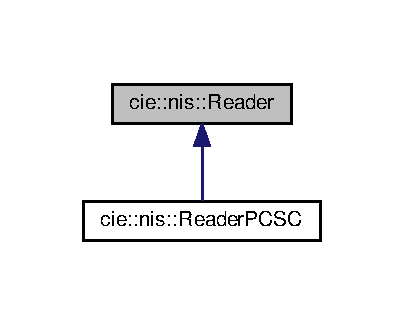
\includegraphics[width=194pt]{classcie_1_1nis_1_1Reader__inherit__graph}
\end{center}
\end{figure}
\subsection*{Public Member Functions}
\begin{DoxyCompactItemize}
\item 
virtual \hyperlink{classcie_1_1nis_1_1Reader_aaca585569e44593b0f56818604336016}{$\sim$\-Reader} ()=0
\item 
virtual \hyperlink{nis__types_8h_a484156f5b8cf43396c5bbe77226fa8da}{Reader\-Result} \hyperlink{classcie_1_1nis_1_1Reader_adcb144784f8ea7c24af4a3f60b47b73d}{enumerate\-Reader\-List} ()=0
\item 
virtual vector$<$ string $>$ \hyperlink{classcie_1_1nis_1_1Reader_adaa0e8d0e2b367c0af8053fde8ae0af8}{get\-Reader\-List} ()=0
\item 
shared\-\_\-ptr$<$ \hyperlink{classcie_1_1nis_1_1Token}{Token} $>$ \hyperlink{classcie_1_1nis_1_1Reader_a40efb63e999b4a53b56a9f3999e884bb}{get\-Token} (const string \&name)
\end{DoxyCompactItemize}
\subsection*{Protected Attributes}
\begin{DoxyCompactItemize}
\item 
unordered\-\_\-map$<$ string, \\*
shared\-\_\-ptr$<$ \hyperlink{classcie_1_1nis_1_1Token}{Token} $>$ $>$ \hyperlink{classcie_1_1nis_1_1Reader_ad94db6ba461e4f00d53488c4863cda20}{token\-List}
\end{DoxyCompactItemize}


\subsection{Constructor \& Destructor Documentation}
\hypertarget{classcie_1_1nis_1_1Reader_aaca585569e44593b0f56818604336016}{\index{cie\-::nis\-::\-Reader@{cie\-::nis\-::\-Reader}!$\sim$\-Reader@{$\sim$\-Reader}}
\index{$\sim$\-Reader@{$\sim$\-Reader}!cie::nis::Reader@{cie\-::nis\-::\-Reader}}
\subsubsection[{$\sim$\-Reader}]{\setlength{\rightskip}{0pt plus 5cm}cie\-::nis\-::\-Reader\-::$\sim$\-Reader (
\begin{DoxyParamCaption}
{}
\end{DoxyParamCaption}
)\hspace{0.3cm}{\ttfamily [pure virtual]}}}\label{classcie_1_1nis_1_1Reader_aaca585569e44593b0f56818604336016}
destructor extending this class should release all associated resources, that's why it's declared pure virtual 

\subsection{Member Function Documentation}
\hypertarget{classcie_1_1nis_1_1Reader_adcb144784f8ea7c24af4a3f60b47b73d}{\index{cie\-::nis\-::\-Reader@{cie\-::nis\-::\-Reader}!enumerate\-Reader\-List@{enumerate\-Reader\-List}}
\index{enumerate\-Reader\-List@{enumerate\-Reader\-List}!cie::nis::Reader@{cie\-::nis\-::\-Reader}}
\subsubsection[{enumerate\-Reader\-List}]{\setlength{\rightskip}{0pt plus 5cm}virtual {\bf Reader\-Result} cie\-::nis\-::\-Reader\-::enumerate\-Reader\-List (
\begin{DoxyParamCaption}
{}
\end{DoxyParamCaption}
)\hspace{0.3cm}{\ttfamily [pure virtual]}}}\label{classcie_1_1nis_1_1Reader_adcb144784f8ea7c24af4a3f60b47b73d}
Add to token\-List the reader compatible with this implementation. \begin{DoxyReturn}{Returns}
\hyperlink{nis__types_8h_a484156f5b8cf43396c5bbe77226fa8da}{Reader\-Result} indicating the success or error 
\end{DoxyReturn}


Implemented in \hyperlink{classcie_1_1nis_1_1ReaderPCSC_a56fcc4887491509d7ae634f89d18a8d6}{cie\-::nis\-::\-Reader\-P\-C\-S\-C}.

\hypertarget{classcie_1_1nis_1_1Reader_adaa0e8d0e2b367c0af8053fde8ae0af8}{\index{cie\-::nis\-::\-Reader@{cie\-::nis\-::\-Reader}!get\-Reader\-List@{get\-Reader\-List}}
\index{get\-Reader\-List@{get\-Reader\-List}!cie::nis::Reader@{cie\-::nis\-::\-Reader}}
\subsubsection[{get\-Reader\-List}]{\setlength{\rightskip}{0pt plus 5cm}virtual vector$<$string$>$ cie\-::nis\-::\-Reader\-::get\-Reader\-List (
\begin{DoxyParamCaption}
{}
\end{DoxyParamCaption}
)\hspace{0.3cm}{\ttfamily [pure virtual]}}}\label{classcie_1_1nis_1_1Reader_adaa0e8d0e2b367c0af8053fde8ae0af8}
Obtain the array of all compatible readers. \begin{DoxyReturn}{Returns}
The array of all the readers managed by this backend 
\end{DoxyReturn}


Implemented in \hyperlink{classcie_1_1nis_1_1ReaderPCSC_a696551fbfc3e27e5f8ea6f4118540bad}{cie\-::nis\-::\-Reader\-P\-C\-S\-C}.

\hypertarget{classcie_1_1nis_1_1Reader_a40efb63e999b4a53b56a9f3999e884bb}{\index{cie\-::nis\-::\-Reader@{cie\-::nis\-::\-Reader}!get\-Token@{get\-Token}}
\index{get\-Token@{get\-Token}!cie::nis::Reader@{cie\-::nis\-::\-Reader}}
\subsubsection[{get\-Token}]{\setlength{\rightskip}{0pt plus 5cm}shared\-\_\-ptr$<${\bf Token}$>$ cie\-::nis\-::\-Reader\-::get\-Token (
\begin{DoxyParamCaption}
\item[{const string \&}]{name}
\end{DoxyParamCaption}
)\hspace{0.3cm}{\ttfamily [inline]}}}\label{classcie_1_1nis_1_1Reader_a40efb63e999b4a53b56a9f3999e884bb}
Obtain a token given its name. \mbox{[}in\mbox{]} name the name of the token as enumerated in \hyperlink{classcie_1_1nis_1_1Reader_adaa0e8d0e2b367c0af8053fde8ae0af8}{get\-Reader\-List()} \begin{DoxyReturn}{Returns}
A reference to the specified \hyperlink{classcie_1_1nis_1_1Token}{Token}, or nullptr if there's no token with that name 
\end{DoxyReturn}


\subsection{Member Data Documentation}
\hypertarget{classcie_1_1nis_1_1Reader_ad94db6ba461e4f00d53488c4863cda20}{\index{cie\-::nis\-::\-Reader@{cie\-::nis\-::\-Reader}!token\-List@{token\-List}}
\index{token\-List@{token\-List}!cie::nis::Reader@{cie\-::nis\-::\-Reader}}
\subsubsection[{token\-List}]{\setlength{\rightskip}{0pt plus 5cm}unordered\-\_\-map$<$string,shared\-\_\-ptr$<${\bf Token}$>$ $>$ cie\-::nis\-::\-Reader\-::token\-List\hspace{0.3cm}{\ttfamily [protected]}}}\label{classcie_1_1nis_1_1Reader_ad94db6ba461e4f00d53488c4863cda20}
the list of the token managed by this backend 

The documentation for this class was generated from the following files\-:\begin{DoxyCompactItemize}
\item 
/home/travis/build/italia/cie-\/nis-\/cpp-\/sdk/src/\hyperlink{reader_8h}{reader.\-h}\item 
/home/travis/build/italia/cie-\/nis-\/cpp-\/sdk/src/reader.\-cpp\end{DoxyCompactItemize}

\hypertarget{classcie_1_1nis_1_1ReaderPCSC}{\section{cie\-:\-:nis\-:\-:Reader\-P\-C\-S\-C Class Reference}
\label{classcie_1_1nis_1_1ReaderPCSC}\index{cie\-::nis\-::\-Reader\-P\-C\-S\-C@{cie\-::nis\-::\-Reader\-P\-C\-S\-C}}
}


Inheritance diagram for cie\-:\-:nis\-:\-:Reader\-P\-C\-S\-C\-:
\nopagebreak
\begin{figure}[H]
\begin{center}
\leavevmode
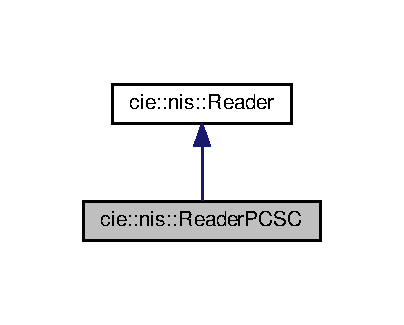
\includegraphics[width=194pt]{classcie_1_1nis_1_1ReaderPCSC__inherit__graph}
\end{center}
\end{figure}


Collaboration diagram for cie\-:\-:nis\-:\-:Reader\-P\-C\-S\-C\-:
\nopagebreak
\begin{figure}[H]
\begin{center}
\leavevmode
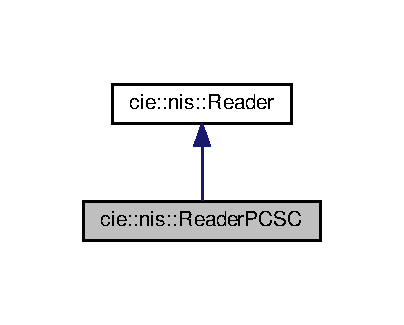
\includegraphics[width=194pt]{classcie_1_1nis_1_1ReaderPCSC__coll__graph}
\end{center}
\end{figure}
\subsection*{Public Member Functions}
\begin{DoxyCompactItemize}
\item 
\hyperlink{nis__types_8h_a484156f5b8cf43396c5bbe77226fa8da}{Reader\-Result} \hyperlink{classcie_1_1nis_1_1ReaderPCSC_a56fcc4887491509d7ae634f89d18a8d6}{enumerate\-Reader\-List} ()
\item 
vector$<$ string $>$ \hyperlink{classcie_1_1nis_1_1ReaderPCSC_a696551fbfc3e27e5f8ea6f4118540bad}{get\-Reader\-List} ()
\item 
\hypertarget{classcie_1_1nis_1_1ReaderPCSC_a60f719d3f0216de1528a031747972257}{bool {\bfseries has\-Context} ()}\label{classcie_1_1nis_1_1ReaderPCSC_a60f719d3f0216de1528a031747972257}

\end{DoxyCompactItemize}
\subsection*{Additional Inherited Members}


\subsection{Member Function Documentation}
\hypertarget{classcie_1_1nis_1_1ReaderPCSC_a56fcc4887491509d7ae634f89d18a8d6}{\index{cie\-::nis\-::\-Reader\-P\-C\-S\-C@{cie\-::nis\-::\-Reader\-P\-C\-S\-C}!enumerate\-Reader\-List@{enumerate\-Reader\-List}}
\index{enumerate\-Reader\-List@{enumerate\-Reader\-List}!cie::nis::ReaderPCSC@{cie\-::nis\-::\-Reader\-P\-C\-S\-C}}
\subsubsection[{enumerate\-Reader\-List}]{\setlength{\rightskip}{0pt plus 5cm}{\bf Reader\-Result} Reader\-P\-C\-S\-C\-::enumerate\-Reader\-List (
\begin{DoxyParamCaption}
{}
\end{DoxyParamCaption}
)\hspace{0.3cm}{\ttfamily [virtual]}}}\label{classcie_1_1nis_1_1ReaderPCSC_a56fcc4887491509d7ae634f89d18a8d6}
Add to token\-List the reader compatible with this implementation. \begin{DoxyReturn}{Returns}
\hyperlink{nis__types_8h_a484156f5b8cf43396c5bbe77226fa8da}{Reader\-Result} indicating the success or error 
\end{DoxyReturn}


Implements \hyperlink{classcie_1_1nis_1_1Reader_adcb144784f8ea7c24af4a3f60b47b73d}{cie\-::nis\-::\-Reader}.

\hypertarget{classcie_1_1nis_1_1ReaderPCSC_a696551fbfc3e27e5f8ea6f4118540bad}{\index{cie\-::nis\-::\-Reader\-P\-C\-S\-C@{cie\-::nis\-::\-Reader\-P\-C\-S\-C}!get\-Reader\-List@{get\-Reader\-List}}
\index{get\-Reader\-List@{get\-Reader\-List}!cie::nis::ReaderPCSC@{cie\-::nis\-::\-Reader\-P\-C\-S\-C}}
\subsubsection[{get\-Reader\-List}]{\setlength{\rightskip}{0pt plus 5cm}vector$<$ string $>$ Reader\-P\-C\-S\-C\-::get\-Reader\-List (
\begin{DoxyParamCaption}
{}
\end{DoxyParamCaption}
)\hspace{0.3cm}{\ttfamily [virtual]}}}\label{classcie_1_1nis_1_1ReaderPCSC_a696551fbfc3e27e5f8ea6f4118540bad}
Obtain the array of all compatible readers. \begin{DoxyReturn}{Returns}
The array of all the readers managed by this backend 
\end{DoxyReturn}


Implements \hyperlink{classcie_1_1nis_1_1Reader_adaa0e8d0e2b367c0af8053fde8ae0af8}{cie\-::nis\-::\-Reader}.



The documentation for this class was generated from the following files\-:\begin{DoxyCompactItemize}
\item 
/home/travis/build/italia/cie-\/nis-\/cpp-\/sdk/src/reader\-\_\-pcsc.\-h\item 
/home/travis/build/italia/cie-\/nis-\/cpp-\/sdk/src/reader\-\_\-pcsc.\-cpp\end{DoxyCompactItemize}

\hypertarget{classcie_1_1nis_1_1Token}{\section{cie\-:\-:nis\-:\-:Token Class Reference}
\label{classcie_1_1nis_1_1Token}\index{cie\-::nis\-::\-Token@{cie\-::nis\-::\-Token}}
}


Inheritance diagram for cie\-:\-:nis\-:\-:Token\-:
\nopagebreak
\begin{figure}[H]
\begin{center}
\leavevmode
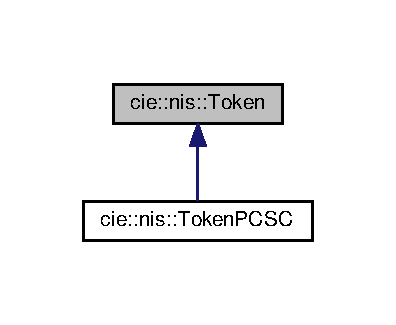
\includegraphics[width=190pt]{classcie_1_1nis_1_1Token__inherit__graph}
\end{center}
\end{figure}
\subsection*{Public Member Functions}
\begin{DoxyCompactItemize}
\item 
\hypertarget{classcie_1_1nis_1_1Token_ae677403b3b8074b908cb416741f93e9e}{int {\bfseries read\-Nis} (char $\ast$const nis\-Data, \hyperlink{nis__types_8h_a01a69b218db702baa14290be05ef112d}{nis\-\_\-callback\-\_\-t} callback, uint32\-\_\-t interval, uint32\-\_\-t $\ast$uid)}\label{classcie_1_1nis_1_1Token_ae677403b3b8074b908cb416741f93e9e}

\item 
\hypertarget{classcie_1_1nis_1_1Token_a3c246d7e4a06c864bcadc6db97d1870e}{std\-::string {\bfseries read\-Nis} ()}\label{classcie_1_1nis_1_1Token_a3c246d7e4a06c864bcadc6db97d1870e}

\item 
\hypertarget{classcie_1_1nis_1_1Token_ab9147907b6d02c2361c2df2212d17a4d}{int {\bfseries configure} (uint32\-\_\-t config)}\label{classcie_1_1nis_1_1Token_ab9147907b6d02c2361c2df2212d17a4d}

\item 
\hypertarget{classcie_1_1nis_1_1Token_a249238a0e7a79237d443bb42bee06b6f}{int {\bfseries reset} ()}\label{classcie_1_1nis_1_1Token_a249238a0e7a79237d443bb42bee06b6f}

\item 
virtual \hyperlink{nis__types_8h_a6ef53483e8ce2f8bc58bd1f75b3d0b38}{Tok\-Result} \hyperlink{classcie_1_1nis_1_1Token_ab7a55406f6b9b15a39d70e64bab0042f}{connect} ()=0
\item 
virtual \hyperlink{nis__types_8h_a6ef53483e8ce2f8bc58bd1f75b3d0b38}{Tok\-Result} \hyperlink{classcie_1_1nis_1_1Token_a851b111864dade8826daa21920fa7cdf}{disconnect} ()=0
\item 
virtual \hyperlink{nis__types_8h_a6ef53483e8ce2f8bc58bd1f75b3d0b38}{Tok\-Result} \hyperlink{classcie_1_1nis_1_1Token_a90c1d8936133fc35b1826b7eebbd13ff}{transmit} (const std\-::vector$<$ B\-Y\-T\-E $>$ \&apdu, std\-::vector$<$ B\-Y\-T\-E $>$ \&response) const =0
\end{DoxyCompactItemize}


\subsection{Member Function Documentation}
\hypertarget{classcie_1_1nis_1_1Token_ab7a55406f6b9b15a39d70e64bab0042f}{\index{cie\-::nis\-::\-Token@{cie\-::nis\-::\-Token}!connect@{connect}}
\index{connect@{connect}!cie::nis::Token@{cie\-::nis\-::\-Token}}
\subsubsection[{connect}]{\setlength{\rightskip}{0pt plus 5cm}virtual {\bf Tok\-Result} cie\-::nis\-::\-Token\-::connect (
\begin{DoxyParamCaption}
{}
\end{DoxyParamCaption}
)\hspace{0.3cm}{\ttfamily [pure virtual]}}}\label{classcie_1_1nis_1_1Token_ab7a55406f6b9b15a39d70e64bab0042f}
Connect to this instance of a token \begin{DoxyReturn}{Returns}
\hyperlink{nis__types_8h_a6ef53483e8ce2f8bc58bd1f75b3d0b38}{Tok\-Result} representing the success or error conditiona 
\end{DoxyReturn}
\begin{DoxySeeAlso}{See Also}
\hyperlink{classcie_1_1nis_1_1Token_a851b111864dade8826daa21920fa7cdf}{disconnect()} 
\end{DoxySeeAlso}


Implemented in \hyperlink{classcie_1_1nis_1_1TokenPCSC_a7078555ef89f4388fa32b60d56d14437}{cie\-::nis\-::\-Token\-P\-C\-S\-C}.

\hypertarget{classcie_1_1nis_1_1Token_a851b111864dade8826daa21920fa7cdf}{\index{cie\-::nis\-::\-Token@{cie\-::nis\-::\-Token}!disconnect@{disconnect}}
\index{disconnect@{disconnect}!cie::nis::Token@{cie\-::nis\-::\-Token}}
\subsubsection[{disconnect}]{\setlength{\rightskip}{0pt plus 5cm}virtual {\bf Tok\-Result} cie\-::nis\-::\-Token\-::disconnect (
\begin{DoxyParamCaption}
{}
\end{DoxyParamCaption}
)\hspace{0.3cm}{\ttfamily [pure virtual]}}}\label{classcie_1_1nis_1_1Token_a851b111864dade8826daa21920fa7cdf}
Disconnect to this instance of a token \begin{DoxyReturn}{Returns}
\hyperlink{nis__types_8h_a6ef53483e8ce2f8bc58bd1f75b3d0b38}{Tok\-Result} representing the success or error conditiona 
\end{DoxyReturn}
\begin{DoxySeeAlso}{See Also}
\hyperlink{classcie_1_1nis_1_1Token_ab7a55406f6b9b15a39d70e64bab0042f}{connect()} 
\end{DoxySeeAlso}


Implemented in \hyperlink{classcie_1_1nis_1_1TokenPCSC_af95dd044db07754ff4ee09e186821fa2}{cie\-::nis\-::\-Token\-P\-C\-S\-C}.

\hypertarget{classcie_1_1nis_1_1Token_a90c1d8936133fc35b1826b7eebbd13ff}{\index{cie\-::nis\-::\-Token@{cie\-::nis\-::\-Token}!transmit@{transmit}}
\index{transmit@{transmit}!cie::nis::Token@{cie\-::nis\-::\-Token}}
\subsubsection[{transmit}]{\setlength{\rightskip}{0pt plus 5cm}virtual {\bf Tok\-Result} cie\-::nis\-::\-Token\-::transmit (
\begin{DoxyParamCaption}
\item[{const std\-::vector$<$ B\-Y\-T\-E $>$ \&}]{apdu, }
\item[{std\-::vector$<$ B\-Y\-T\-E $>$ \&}]{response}
\end{DoxyParamCaption}
) const\hspace{0.3cm}{\ttfamily [pure virtual]}}}\label{classcie_1_1nis_1_1Token_a90c1d8936133fc35b1826b7eebbd13ff}
Transmit a specific apdu to a card and obtain its response 
\begin{DoxyParams}[1]{Parameters}
\mbox{\tt in}  & {\em array} & containing the apdu to be sent to the token \\
\hline
\mbox{\tt out}  & {\em the} & response sent from the token \\
\hline
\end{DoxyParams}
\begin{DoxyReturn}{Returns}
\hyperlink{nis__types_8h_a6ef53483e8ce2f8bc58bd1f75b3d0b38}{Tok\-Result} representing the success or error condition 
\end{DoxyReturn}


Implemented in \hyperlink{classcie_1_1nis_1_1TokenPCSC_a23176a026828460420ea3e9619c7664d}{cie\-::nis\-::\-Token\-P\-C\-S\-C}.



The documentation for this class was generated from the following files\-:\begin{DoxyCompactItemize}
\item 
/home/travis/build/italia/cie-\/nis-\/cpp-\/sdk/src/\hyperlink{token_8h}{token.\-h}\item 
/home/travis/build/italia/cie-\/nis-\/cpp-\/sdk/src/token.\-cpp\end{DoxyCompactItemize}

\hypertarget{classcie_1_1nis_1_1TokenPCSC}{\section{cie\-:\-:nis\-:\-:Token\-P\-C\-S\-C Class Reference}
\label{classcie_1_1nis_1_1TokenPCSC}\index{cie\-::nis\-::\-Token\-P\-C\-S\-C@{cie\-::nis\-::\-Token\-P\-C\-S\-C}}
}


Inheritance diagram for cie\-:\-:nis\-:\-:Token\-P\-C\-S\-C\-:
\nopagebreak
\begin{figure}[H]
\begin{center}
\leavevmode
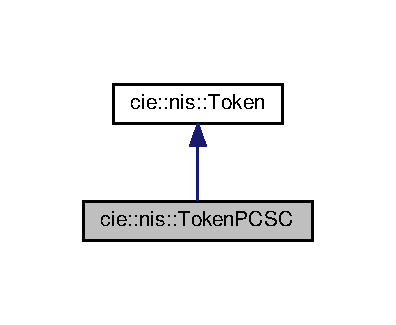
\includegraphics[width=190pt]{classcie_1_1nis_1_1TokenPCSC__inherit__graph}
\end{center}
\end{figure}


Collaboration diagram for cie\-:\-:nis\-:\-:Token\-P\-C\-S\-C\-:
\nopagebreak
\begin{figure}[H]
\begin{center}
\leavevmode
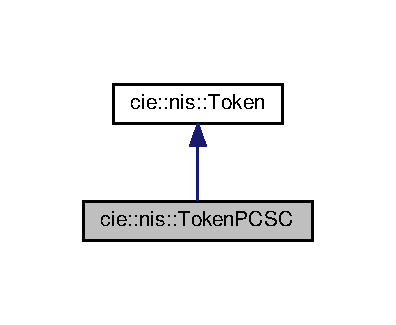
\includegraphics[width=190pt]{classcie_1_1nis_1_1TokenPCSC__coll__graph}
\end{center}
\end{figure}
\subsection*{Public Member Functions}
\begin{DoxyCompactItemize}
\item 
\hypertarget{classcie_1_1nis_1_1TokenPCSC_ae72b5cf6f97ab41d4a95f87c3a3fa8cc}{{\bfseries Token\-P\-C\-S\-C} (const string \&identifier, S\-C\-A\-R\-D\-C\-O\-N\-T\-E\-X\-T context)}\label{classcie_1_1nis_1_1TokenPCSC_ae72b5cf6f97ab41d4a95f87c3a3fa8cc}

\item 
\hyperlink{nis__types_8h_a6ef53483e8ce2f8bc58bd1f75b3d0b38}{Tok\-Result} \hyperlink{classcie_1_1nis_1_1TokenPCSC_a7078555ef89f4388fa32b60d56d14437}{connect} ()
\item 
\hyperlink{nis__types_8h_a6ef53483e8ce2f8bc58bd1f75b3d0b38}{Tok\-Result} \hyperlink{classcie_1_1nis_1_1TokenPCSC_af95dd044db07754ff4ee09e186821fa2}{disconnect} ()
\item 
\hyperlink{nis__types_8h_a6ef53483e8ce2f8bc58bd1f75b3d0b38}{Tok\-Result} \hyperlink{classcie_1_1nis_1_1TokenPCSC_a23176a026828460420ea3e9619c7664d}{transmit} (const std\-::vector$<$ B\-Y\-T\-E $>$ \&apdu, std\-::vector$<$ B\-Y\-T\-E $>$ \&response) const 
\end{DoxyCompactItemize}


\subsection{Member Function Documentation}
\hypertarget{classcie_1_1nis_1_1TokenPCSC_a7078555ef89f4388fa32b60d56d14437}{\index{cie\-::nis\-::\-Token\-P\-C\-S\-C@{cie\-::nis\-::\-Token\-P\-C\-S\-C}!connect@{connect}}
\index{connect@{connect}!cie::nis::TokenPCSC@{cie\-::nis\-::\-Token\-P\-C\-S\-C}}
\subsubsection[{connect}]{\setlength{\rightskip}{0pt plus 5cm}{\bf Tok\-Result} Token\-P\-C\-S\-C\-::connect (
\begin{DoxyParamCaption}
{}
\end{DoxyParamCaption}
)\hspace{0.3cm}{\ttfamily [virtual]}}}\label{classcie_1_1nis_1_1TokenPCSC_a7078555ef89f4388fa32b60d56d14437}
Connect to this instance of a token \begin{DoxyReturn}{Returns}
\hyperlink{nis__types_8h_a6ef53483e8ce2f8bc58bd1f75b3d0b38}{Tok\-Result} representing the success or error conditiona 
\end{DoxyReturn}
\begin{DoxySeeAlso}{See Also}
\hyperlink{classcie_1_1nis_1_1TokenPCSC_af95dd044db07754ff4ee09e186821fa2}{disconnect()} 
\end{DoxySeeAlso}


Implements \hyperlink{classcie_1_1nis_1_1Token_ab7a55406f6b9b15a39d70e64bab0042f}{cie\-::nis\-::\-Token}.

\hypertarget{classcie_1_1nis_1_1TokenPCSC_af95dd044db07754ff4ee09e186821fa2}{\index{cie\-::nis\-::\-Token\-P\-C\-S\-C@{cie\-::nis\-::\-Token\-P\-C\-S\-C}!disconnect@{disconnect}}
\index{disconnect@{disconnect}!cie::nis::TokenPCSC@{cie\-::nis\-::\-Token\-P\-C\-S\-C}}
\subsubsection[{disconnect}]{\setlength{\rightskip}{0pt plus 5cm}{\bf Tok\-Result} Token\-P\-C\-S\-C\-::disconnect (
\begin{DoxyParamCaption}
{}
\end{DoxyParamCaption}
)\hspace{0.3cm}{\ttfamily [virtual]}}}\label{classcie_1_1nis_1_1TokenPCSC_af95dd044db07754ff4ee09e186821fa2}
Disconnect to this instance of a token \begin{DoxyReturn}{Returns}
\hyperlink{nis__types_8h_a6ef53483e8ce2f8bc58bd1f75b3d0b38}{Tok\-Result} representing the success or error conditiona 
\end{DoxyReturn}
\begin{DoxySeeAlso}{See Also}
\hyperlink{classcie_1_1nis_1_1TokenPCSC_a7078555ef89f4388fa32b60d56d14437}{connect()} 
\end{DoxySeeAlso}


Implements \hyperlink{classcie_1_1nis_1_1Token_a851b111864dade8826daa21920fa7cdf}{cie\-::nis\-::\-Token}.

\hypertarget{classcie_1_1nis_1_1TokenPCSC_a23176a026828460420ea3e9619c7664d}{\index{cie\-::nis\-::\-Token\-P\-C\-S\-C@{cie\-::nis\-::\-Token\-P\-C\-S\-C}!transmit@{transmit}}
\index{transmit@{transmit}!cie::nis::TokenPCSC@{cie\-::nis\-::\-Token\-P\-C\-S\-C}}
\subsubsection[{transmit}]{\setlength{\rightskip}{0pt plus 5cm}{\bf Tok\-Result} Token\-P\-C\-S\-C\-::transmit (
\begin{DoxyParamCaption}
\item[{const std\-::vector$<$ B\-Y\-T\-E $>$ \&}]{apdu, }
\item[{std\-::vector$<$ B\-Y\-T\-E $>$ \&}]{response}
\end{DoxyParamCaption}
) const\hspace{0.3cm}{\ttfamily [virtual]}}}\label{classcie_1_1nis_1_1TokenPCSC_a23176a026828460420ea3e9619c7664d}
Transmit a specific apdu to a card and obtain its response 
\begin{DoxyParams}[1]{Parameters}
\mbox{\tt in}  & {\em array} & containing the apdu to be sent to the token \\
\hline
\mbox{\tt out}  & {\em the} & response sent from the token \\
\hline
\end{DoxyParams}
\begin{DoxyReturn}{Returns}
\hyperlink{nis__types_8h_a6ef53483e8ce2f8bc58bd1f75b3d0b38}{Tok\-Result} representing the success or error condition 
\end{DoxyReturn}


Implements \hyperlink{classcie_1_1nis_1_1Token_a90c1d8936133fc35b1826b7eebbd13ff}{cie\-::nis\-::\-Token}.



The documentation for this class was generated from the following files\-:\begin{DoxyCompactItemize}
\item 
/home/travis/build/italia/cie-\/nis-\/cpp-\/sdk/src/token\-\_\-pcsc.\-h\item 
/home/travis/build/italia/cie-\/nis-\/cpp-\/sdk/src/token\-\_\-pcsc.\-cpp\end{DoxyCompactItemize}

\hypertarget{classUtils}{\section{Utils Class Reference}
\label{classUtils}\index{Utils@{Utils}}
}
\subsection*{Static Public Member Functions}
\begin{DoxyCompactItemize}
\item 
static uint32\-\_\-t \hyperlink{classUtils_a530a848112e369976fe29b2310eb3302}{get\-Uid} ()
\end{DoxyCompactItemize}


\subsection{Member Function Documentation}
\hypertarget{classUtils_a530a848112e369976fe29b2310eb3302}{\index{Utils@{Utils}!get\-Uid@{get\-Uid}}
\index{get\-Uid@{get\-Uid}!Utils@{Utils}}
\subsubsection[{get\-Uid}]{\setlength{\rightskip}{0pt plus 5cm}static uint32\-\_\-t Utils\-::get\-Uid (
\begin{DoxyParamCaption}
{}
\end{DoxyParamCaption}
)\hspace{0.3cm}{\ttfamily [inline]}, {\ttfamily [static]}}}\label{classUtils_a530a848112e369976fe29b2310eb3302}
Generates an U\-I\-D \begin{DoxyReturn}{Returns}
the U\-I\-D generated 
\end{DoxyReturn}


The documentation for this class was generated from the following file\-:\begin{DoxyCompactItemize}
\item 
/home/travis/build/italia/cie-\/nis-\/cpp-\/sdk/src/uid.\-h\end{DoxyCompactItemize}

\chapter{File Documentation}
\hypertarget{executor_8h}{\section{/home/travis/build/italia/cie-\/nis-\/cpp-\/sdk/src/executor.h File Reference}
\label{executor_8h}\index{/home/travis/build/italia/cie-\/nis-\/cpp-\/sdk/src/executor.\-h@{/home/travis/build/italia/cie-\/nis-\/cpp-\/sdk/src/executor.\-h}}
}


Executor thread.  


{\ttfamily \#include $<$thread$>$}\\*
{\ttfamily \#include $<$iostream$>$}\\*
{\ttfamily \#include \char`\"{}nis\-\_\-types.\-h\char`\"{}}\\*
Include dependency graph for executor.\-h\-:
\nopagebreak
\begin{figure}[H]
\begin{center}
\leavevmode
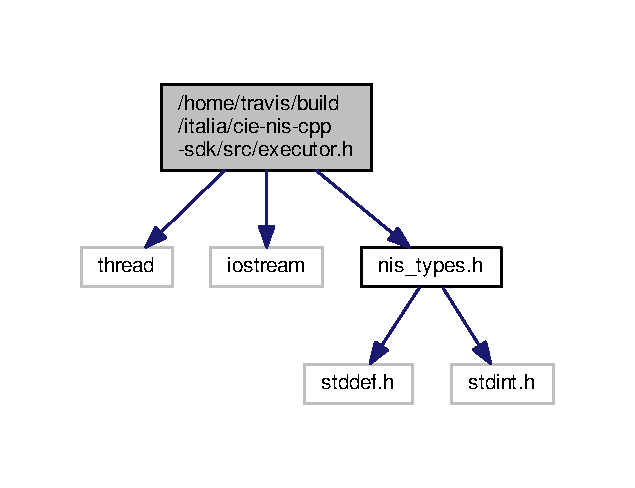
\includegraphics[width=305pt]{executor_8h__incl}
\end{center}
\end{figure}
This graph shows which files directly or indirectly include this file\-:
\nopagebreak
\begin{figure}[H]
\begin{center}
\leavevmode
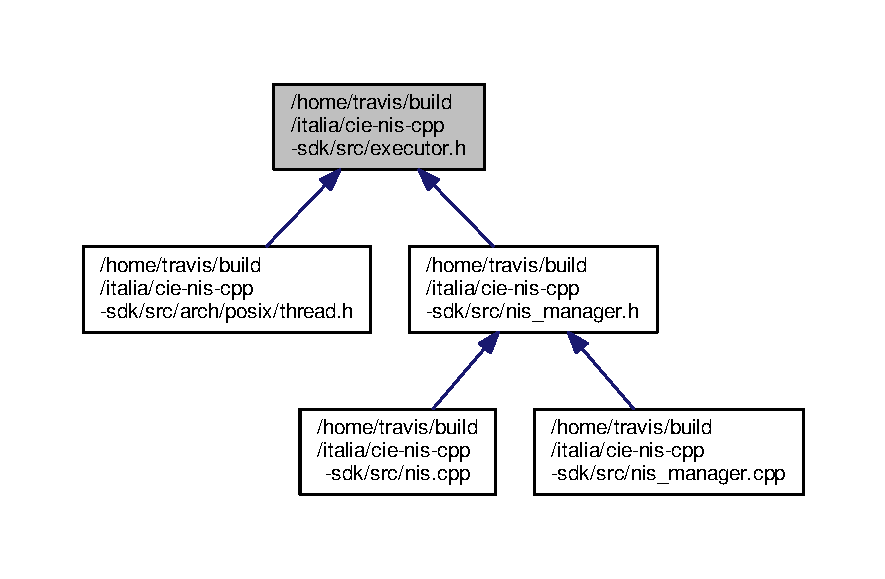
\includegraphics[width=350pt]{executor_8h__dep__incl}
\end{center}
\end{figure}
\subsection*{Classes}
\begin{DoxyCompactItemize}
\item 
struct \hyperlink{structPollExecutor}{Poll\-Executor}
\end{DoxyCompactItemize}


\subsection{Detailed Description}
Executor thread. An executor allows to perform deferred work on a token 
\hypertarget{nis_8cpp}{\section{/home/travis/build/italia/cie-\/nis-\/cpp-\/sdk/src/nis.cpp File Reference}
\label{nis_8cpp}\index{/home/travis/build/italia/cie-\/nis-\/cpp-\/sdk/src/nis.\-cpp@{/home/travis/build/italia/cie-\/nis-\/cpp-\/sdk/src/nis.\-cpp}}
}


Main facilities.  


{\ttfamily \#include \char`\"{}nis.\-h\char`\"{}}\\*
{\ttfamily \#include $<$unordered\-\_\-map$>$}\\*
{\ttfamily \#include $<$vector$>$}\\*
{\ttfamily \#include $<$thread$>$}\\*
{\ttfamily \#include $<$mutex$>$}\\*
{\ttfamily \#include $<$functional$>$}\\*
{\ttfamily \#include $<$cstring$>$}\\*
{\ttfamily \#include $<$algorithm$>$}\\*
{\ttfamily \#include \char`\"{}reader.\-h\char`\"{}}\\*
{\ttfamily \#include \char`\"{}reader\-\_\-pcsc.\-h\char`\"{}}\\*
{\ttfamily \#include \char`\"{}token.\-h\char`\"{}}\\*
{\ttfamily \#include \char`\"{}token\-\_\-pcsc.\-h\char`\"{}}\\*
{\ttfamily \#include \char`\"{}requests.\-h\char`\"{}}\\*
{\ttfamily \#include \char`\"{}thread.\-h\char`\"{}}\\*
{\ttfamily \#include \char`\"{}uid.\-h\char`\"{}}\\*
{\ttfamily \#include \char`\"{}nis\-\_\-manager.\-h\char`\"{}}\\*
Include dependency graph for nis.\-cpp\-:
\nopagebreak
\begin{figure}[H]
\begin{center}
\leavevmode
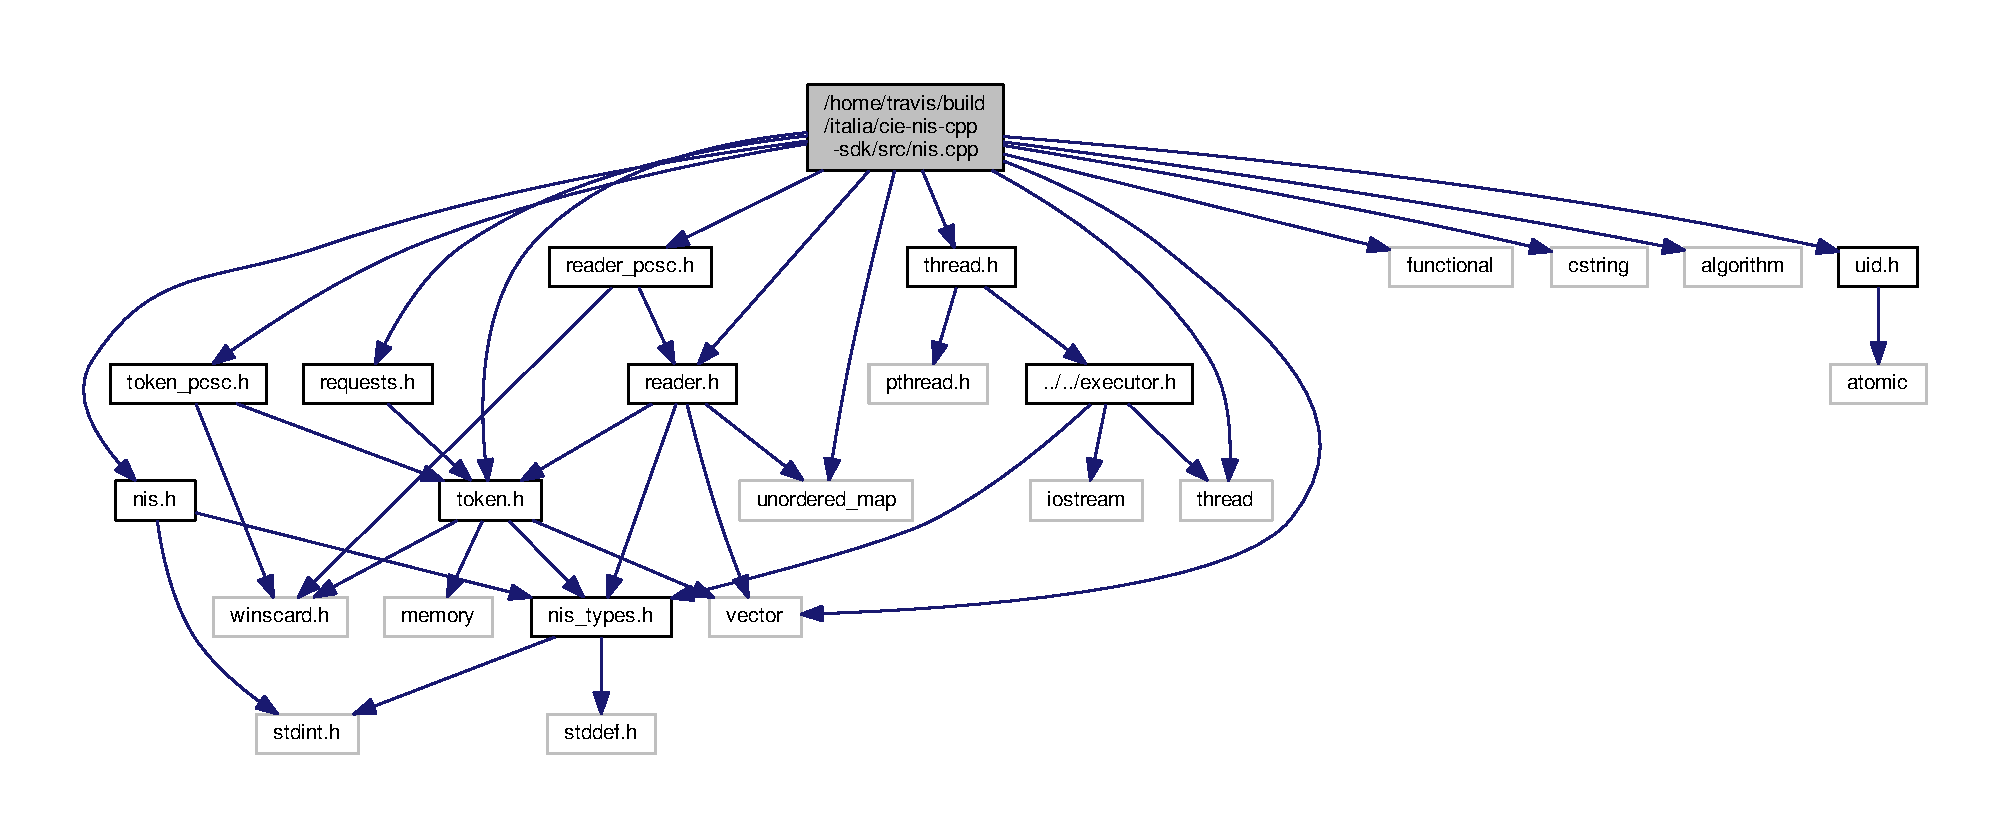
\includegraphics[width=350pt]{nis_8cpp__incl}
\end{center}
\end{figure}
\subsection*{Namespaces}
\begin{DoxyCompactItemize}
\item 
\hyperlink{namespacecie}{cie}
\begin{DoxyCompactList}\small\item\em cie namespace \end{DoxyCompactList}\item 
\hyperlink{namespacecie_1_1nis}{cie\-::nis}
\begin{DoxyCompactList}\small\item\em nis namespace \end{DoxyCompactList}\end{DoxyCompactItemize}
\subsection*{Functions}
\begin{DoxyCompactItemize}
\item 
int \hyperlink{namespacecie_1_1nis_abcdd144762aaa78abbf48a4252ee15e5}{cie\-::nis\-::init} (uint32\-\_\-t backend\-Bitfield)
\item 
vector$<$ string $>$ \hyperlink{namespacecie_1_1nis_a90d4445f8f3cc7ab7ea75b8c70aeaf63}{cie\-::nis\-::readers\-List} ()
\item 
\hyperlink{classcie_1_1nis_1_1Token}{Token} $\ast$ \hyperlink{namespacecie_1_1nis_aadf97fb070ca1d79e93f802d8de769e6}{cie\-::nis\-::get\-Token} (string reader\-Name)
\item 
int \hyperlink{namespacecie_1_1nis_a0c20f013bbac3f773e89a57591af68a9}{cie\-::nis\-::deinit} (uint32\-\_\-t backend\-Bitfield)
\item 
int \hyperlink{namespacecie_1_1nis_aa031abccb193d600ad1cd71b414abafa}{cie\-::nis\-::stop\-Poll} (uint32\-\_\-t uid)
\item 
int \hyperlink{nis_8cpp_a1a4da622cc9443c4fc71b276454923da}{N\-I\-S\-\_\-\-Init} (uint32\-\_\-t backend\-Bitfield)
\item 
int \hyperlink{nis_8cpp_a8a7d97b92e4703b0c539676d98697224}{N\-I\-S\-\_\-\-Reader\-List} (char $\ast$$\ast$readers, size\-\_\-t $\ast$len)
\item 
\hyperlink{nis__types_8h_aeda8757494329f27e534f367b067eda3}{N\-I\-S\-Handle} \hyperlink{nis_8cpp_a580bbcb89dd427ba80c7965e374e47a4}{N\-I\-S\-\_\-\-Get\-Handle} (char $\ast$reader\-Name)
\item 
int \hyperlink{nis_8cpp_adb93e961f1f17f1201604b40313875e0}{N\-I\-S\-\_\-\-Read\-Nis} (\hyperlink{nis__types_8h_aeda8757494329f27e534f367b067eda3}{N\-I\-S\-Handle} handle, char $\ast$const nis\-Data, \hyperlink{nis__types_8h_a01a69b218db702baa14290be05ef112d}{nis\-\_\-callback\-\_\-t} callback, uint32\-\_\-t interval, uint32\-\_\-t $\ast$uid)
\item 
int \hyperlink{nis_8cpp_a209375c2a603b38401c2a75074a7ede4}{N\-I\-S\-\_\-\-Stop\-Poll} (uint32\-\_\-t uid)
\item 
\hypertarget{nis_8cpp_a1f9621bef29cd4cb4c7af129a78cdea4}{int {\bfseries N\-I\-S\-\_\-\-Config\-Handle} (\hyperlink{nis__types_8h_aeda8757494329f27e534f367b067eda3}{N\-I\-S\-Handle} handle, uint32\-\_\-t config)}\label{nis_8cpp_a1f9621bef29cd4cb4c7af129a78cdea4}

\item 
int \hyperlink{nis_8cpp_a1a5442dc5745e4bdde47ff3002f48dca}{N\-I\-S\-\_\-\-Deinit} (uint32\-\_\-t backend\-Bitfield)
\item 
\hypertarget{nis_8cpp_a745181048a1c748d3c662c03a54d0d8c}{int {\bfseries N\-I\-S\-\_\-\-Reset} (\hyperlink{nis__types_8h_aeda8757494329f27e534f367b067eda3}{N\-I\-S\-Handle} handle)}\label{nis_8cpp_a745181048a1c748d3c662c03a54d0d8c}

\end{DoxyCompactItemize}


\subsection{Detailed Description}
Main facilities. This file contains the most important core functions of the entire N\-I\-S sdk. Just include {\itshape \hyperlink{nis_8h_source}{nis.\-h}} in your source code to use this A\-P\-I. 

\subsection{Function Documentation}
\hypertarget{nis_8cpp_a1a5442dc5745e4bdde47ff3002f48dca}{\index{nis.\-cpp@{nis.\-cpp}!N\-I\-S\-\_\-\-Deinit@{N\-I\-S\-\_\-\-Deinit}}
\index{N\-I\-S\-\_\-\-Deinit@{N\-I\-S\-\_\-\-Deinit}!nis.cpp@{nis.\-cpp}}
\subsubsection[{N\-I\-S\-\_\-\-Deinit}]{\setlength{\rightskip}{0pt plus 5cm}int N\-I\-S\-\_\-\-Deinit (
\begin{DoxyParamCaption}
\item[{uint32\-\_\-t}]{backend\-Bitfield}
\end{DoxyParamCaption}
)}}\label{nis_8cpp_a1a5442dc5745e4bdde47ff3002f48dca}
Deinitialize the N\-I\-S sdk backends. Frees all related data, so handlers obtained through \hyperlink{nis_8cpp_a580bbcb89dd427ba80c7965e374e47a4}{N\-I\-S\-\_\-\-Get\-Handle()} or the reader list allocated by \hyperlink{nis_8cpp_a8a7d97b92e4703b0c539676d98697224}{N\-I\-S\-\_\-\-Reader\-List()} are not valid anymore. 
\begin{DoxyParams}[1]{Parameters}
\mbox{\tt in}  & {\em backend\-Bitfield} & Bitfield representing the backends to be deinitialized, taken from \hyperlink{nis__types_8h_acee299fbb7d897867808250049524594}{Backend\-Type} \\
\hline
\end{DoxyParams}
\begin{DoxySeeAlso}{See Also}

\end{DoxySeeAlso}
\begin{DoxyReturn}{Returns}
0 on success, negative on error 
\end{DoxyReturn}
\hypertarget{nis_8cpp_a580bbcb89dd427ba80c7965e374e47a4}{\index{nis.\-cpp@{nis.\-cpp}!N\-I\-S\-\_\-\-Get\-Handle@{N\-I\-S\-\_\-\-Get\-Handle}}
\index{N\-I\-S\-\_\-\-Get\-Handle@{N\-I\-S\-\_\-\-Get\-Handle}!nis.cpp@{nis.\-cpp}}
\subsubsection[{N\-I\-S\-\_\-\-Get\-Handle}]{\setlength{\rightskip}{0pt plus 5cm}{\bf N\-I\-S\-Handle} N\-I\-S\-\_\-\-Get\-Handle (
\begin{DoxyParamCaption}
\item[{char $\ast$}]{reader\-Name}
\end{DoxyParamCaption}
)}}\label{nis_8cpp_a580bbcb89dd427ba80c7965e374e47a4}
Obtain the handler of a specific reader. 
\begin{DoxyParams}[1]{Parameters}
\mbox{\tt in}  & {\em reader\-Name} & a string representing the name of the reader. A list of readers name can be obtain invoking \hyperlink{nis_8cpp_a8a7d97b92e4703b0c539676d98697224}{N\-I\-S\-\_\-\-Reader\-List()} \\
\hline
\end{DoxyParams}
\begin{DoxyReturn}{Returns}
0 on success, negative on error. 
\end{DoxyReturn}
\hypertarget{nis_8cpp_a1a4da622cc9443c4fc71b276454923da}{\index{nis.\-cpp@{nis.\-cpp}!N\-I\-S\-\_\-\-Init@{N\-I\-S\-\_\-\-Init}}
\index{N\-I\-S\-\_\-\-Init@{N\-I\-S\-\_\-\-Init}!nis.cpp@{nis.\-cpp}}
\subsubsection[{N\-I\-S\-\_\-\-Init}]{\setlength{\rightskip}{0pt plus 5cm}int N\-I\-S\-\_\-\-Init (
\begin{DoxyParamCaption}
\item[{uint32\-\_\-t}]{backend\-Bitfield}
\end{DoxyParamCaption}
)}}\label{nis_8cpp_a1a4da622cc9443c4fc71b276454923da}
Initialize the N\-I\-S sdk backends. 
\begin{DoxyParams}[1]{Parameters}
\mbox{\tt in}  & {\em backend\-Bitfield} & Bitfield representing the backends to be initialized, taken from \hyperlink{nis__types_8h_acee299fbb7d897867808250049524594}{Backend\-Type} \\
\hline
\end{DoxyParams}
\begin{DoxySeeAlso}{See Also}

\end{DoxySeeAlso}
\begin{DoxyReturn}{Returns}
0 on success, negative on error 
\end{DoxyReturn}
\hypertarget{nis_8cpp_a8a7d97b92e4703b0c539676d98697224}{\index{nis.\-cpp@{nis.\-cpp}!N\-I\-S\-\_\-\-Reader\-List@{N\-I\-S\-\_\-\-Reader\-List}}
\index{N\-I\-S\-\_\-\-Reader\-List@{N\-I\-S\-\_\-\-Reader\-List}!nis.cpp@{nis.\-cpp}}
\subsubsection[{N\-I\-S\-\_\-\-Reader\-List}]{\setlength{\rightskip}{0pt plus 5cm}int N\-I\-S\-\_\-\-Reader\-List (
\begin{DoxyParamCaption}
\item[{char $\ast$$\ast$}]{readers, }
\item[{size\-\_\-t $\ast$}]{len}
\end{DoxyParamCaption}
)}}\label{nis_8cpp_a8a7d97b92e4703b0c539676d98697224}
Obtain the connected reader list. 
\begin{DoxyParams}[1]{Parameters}
\mbox{\tt out}  & {\em readers} & if the value {\itshape len} points to is 0 then {\itshape readers} will be automatically allocated (and automatically freed on deinit, so no user intervention is required). If not, readers must point to a pointer to a valid array allocated by the caller who is the owner of that array \\
\hline
\mbox{\tt in,out}  & {\em len} & could point to a value of 0 for auto-\/allocation, or to the size of {\itshape readers} array when it's provided by the user \\
\hline
\end{DoxyParams}
\begin{DoxyReturn}{Returns}
0 on success, negative on error. If negative, the abs value stands for the number of backends for which it was not possible to get the reader list 
\end{DoxyReturn}
\hypertarget{nis_8cpp_adb93e961f1f17f1201604b40313875e0}{\index{nis.\-cpp@{nis.\-cpp}!N\-I\-S\-\_\-\-Read\-Nis@{N\-I\-S\-\_\-\-Read\-Nis}}
\index{N\-I\-S\-\_\-\-Read\-Nis@{N\-I\-S\-\_\-\-Read\-Nis}!nis.cpp@{nis.\-cpp}}
\subsubsection[{N\-I\-S\-\_\-\-Read\-Nis}]{\setlength{\rightskip}{0pt plus 5cm}int N\-I\-S\-\_\-\-Read\-Nis (
\begin{DoxyParamCaption}
\item[{{\bf N\-I\-S\-Handle}}]{handle, }
\item[{char $\ast$const}]{nis\-Data, }
\item[{{\bf nis\-\_\-callback\-\_\-t}}]{callback, }
\item[{uint32\-\_\-t}]{interval, }
\item[{uint32\-\_\-t $\ast$}]{uid}
\end{DoxyParamCaption}
)}}\label{nis_8cpp_adb93e961f1f17f1201604b40313875e0}
Read the N\-I\-S from the specified token. 
\begin{DoxyParams}[1]{Parameters}
\mbox{\tt in}  & {\em handle} & the handler of the reader previously obtained calling \hyperlink{nis_8cpp_a580bbcb89dd427ba80c7965e374e47a4}{N\-I\-S\-\_\-\-Get\-Handle()} \\
\hline
\mbox{\tt out}  & {\em nis\-Data} & array in which to store the N\-I\-S read back from the token. Should be long enough to contains the entire nis as a C-\/style sring, i.\-e. 12 (N\-I\-S) + 1 (null terminator) = 13 chars \\
\hline
\mbox{\tt in}  & {\em callback} & if {\itshape N\-U\-L\-L} the call is blocking and the N\-I\-S is copied inside {\itshape nis\-Data} upon return, otherwise the function spawns a background thread and returns immediately. The thread will invoke the callback funcion passing to it the read N\-I\-S \\
\hline
\mbox{\tt in}  & {\em interval} & time in ms between polls \\
\hline
\mbox{\tt out}  & {\em the} & U\-I\-D associated to the newly created context of execution \\
\hline
\end{DoxyParams}
\begin{DoxyReturn}{Returns}
0 on success, negative on error 
\end{DoxyReturn}
\begin{DoxySeeAlso}{See Also}
\hyperlink{nis_8cpp_a209375c2a603b38401c2a75074a7ede4}{N\-I\-S\-\_\-\-Stop\-Poll()} 
\end{DoxySeeAlso}
\hypertarget{nis_8cpp_a209375c2a603b38401c2a75074a7ede4}{\index{nis.\-cpp@{nis.\-cpp}!N\-I\-S\-\_\-\-Stop\-Poll@{N\-I\-S\-\_\-\-Stop\-Poll}}
\index{N\-I\-S\-\_\-\-Stop\-Poll@{N\-I\-S\-\_\-\-Stop\-Poll}!nis.cpp@{nis.\-cpp}}
\subsubsection[{N\-I\-S\-\_\-\-Stop\-Poll}]{\setlength{\rightskip}{0pt plus 5cm}int N\-I\-S\-\_\-\-Stop\-Poll (
\begin{DoxyParamCaption}
\item[{uint32\-\_\-t}]{uid}
\end{DoxyParamCaption}
)}}\label{nis_8cpp_a209375c2a603b38401c2a75074a7ede4}
Stop the polling on a specified reader started invoking \hyperlink{nis_8cpp_adb93e961f1f17f1201604b40313875e0}{N\-I\-S\-\_\-\-Read\-Nis()} with a callback function. 
\begin{DoxyParams}[1]{Parameters}
\mbox{\tt in}  & {\em uid} & the U\-I\-D of the context of execution previously obtained from e.\-g. \hyperlink{nis_8cpp_adb93e961f1f17f1201604b40313875e0}{N\-I\-S\-\_\-\-Read\-Nis()} \\
\hline
\end{DoxyParams}
\begin{DoxyReturn}{Returns}
0 on success, negative on error. 
\end{DoxyReturn}

\hypertarget{nis__manager_8cpp}{\section{/home/travis/build/italia/cie-\/nis-\/cpp-\/sdk/src/nis\-\_\-manager.cpp File Reference}
\label{nis__manager_8cpp}\index{/home/travis/build/italia/cie-\/nis-\/cpp-\/sdk/src/nis\-\_\-manager.\-cpp@{/home/travis/build/italia/cie-\/nis-\/cpp-\/sdk/src/nis\-\_\-manager.\-cpp}}
}


N\-I\-S Manager implementation.  


{\ttfamily \#include \char`\"{}nis\-\_\-manager.\-h\char`\"{}}\\*
Include dependency graph for nis\-\_\-manager.\-cpp\-:
\nopagebreak
\begin{figure}[H]
\begin{center}
\leavevmode
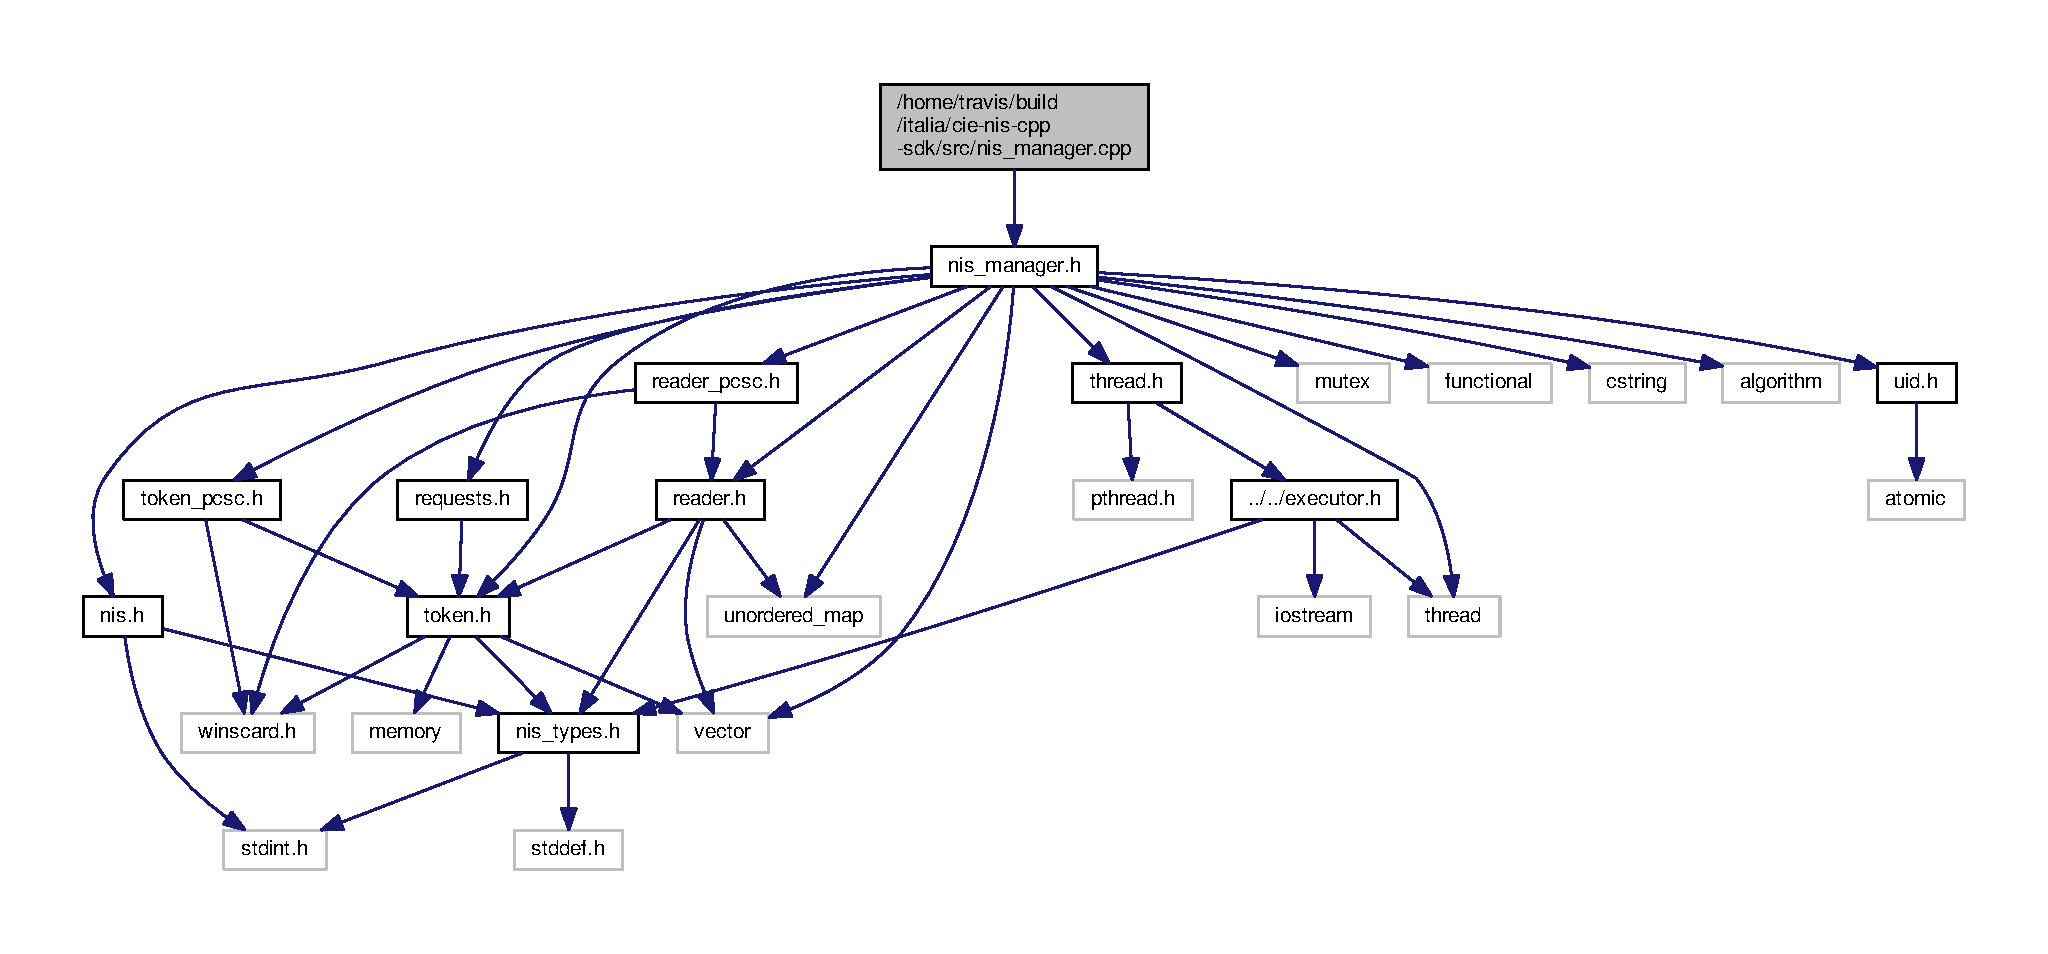
\includegraphics[width=350pt]{nis__manager_8cpp__incl}
\end{center}
\end{figure}


\subsection{Detailed Description}
N\-I\-S Manager implementation. This file contains the implementation of teh N\-I\-S Manager. 
\hypertarget{nis__manager_8h}{\section{/home/travis/build/italia/cie-\/nis-\/cpp-\/sdk/src/nis\-\_\-manager.h File Reference}
\label{nis__manager_8h}\index{/home/travis/build/italia/cie-\/nis-\/cpp-\/sdk/src/nis\-\_\-manager.\-h@{/home/travis/build/italia/cie-\/nis-\/cpp-\/sdk/src/nis\-\_\-manager.\-h}}
}


N\-I\-S Manager.  


{\ttfamily \#include \char`\"{}nis.\-h\char`\"{}}\\*
{\ttfamily \#include $<$unordered\-\_\-map$>$}\\*
{\ttfamily \#include $<$vector$>$}\\*
{\ttfamily \#include $<$thread$>$}\\*
{\ttfamily \#include $<$mutex$>$}\\*
{\ttfamily \#include $<$functional$>$}\\*
{\ttfamily \#include $<$cstring$>$}\\*
{\ttfamily \#include $<$algorithm$>$}\\*
{\ttfamily \#include \char`\"{}reader.\-h\char`\"{}}\\*
{\ttfamily \#include \char`\"{}reader\-\_\-pcsc.\-h\char`\"{}}\\*
{\ttfamily \#include \char`\"{}token.\-h\char`\"{}}\\*
{\ttfamily \#include \char`\"{}token\-\_\-pcsc.\-h\char`\"{}}\\*
{\ttfamily \#include \char`\"{}requests.\-h\char`\"{}}\\*
{\ttfamily \#include \char`\"{}thread.\-h\char`\"{}}\\*
{\ttfamily \#include \char`\"{}uid.\-h\char`\"{}}\\*
Include dependency graph for nis\-\_\-manager.\-h\-:
\nopagebreak
\begin{figure}[H]
\begin{center}
\leavevmode
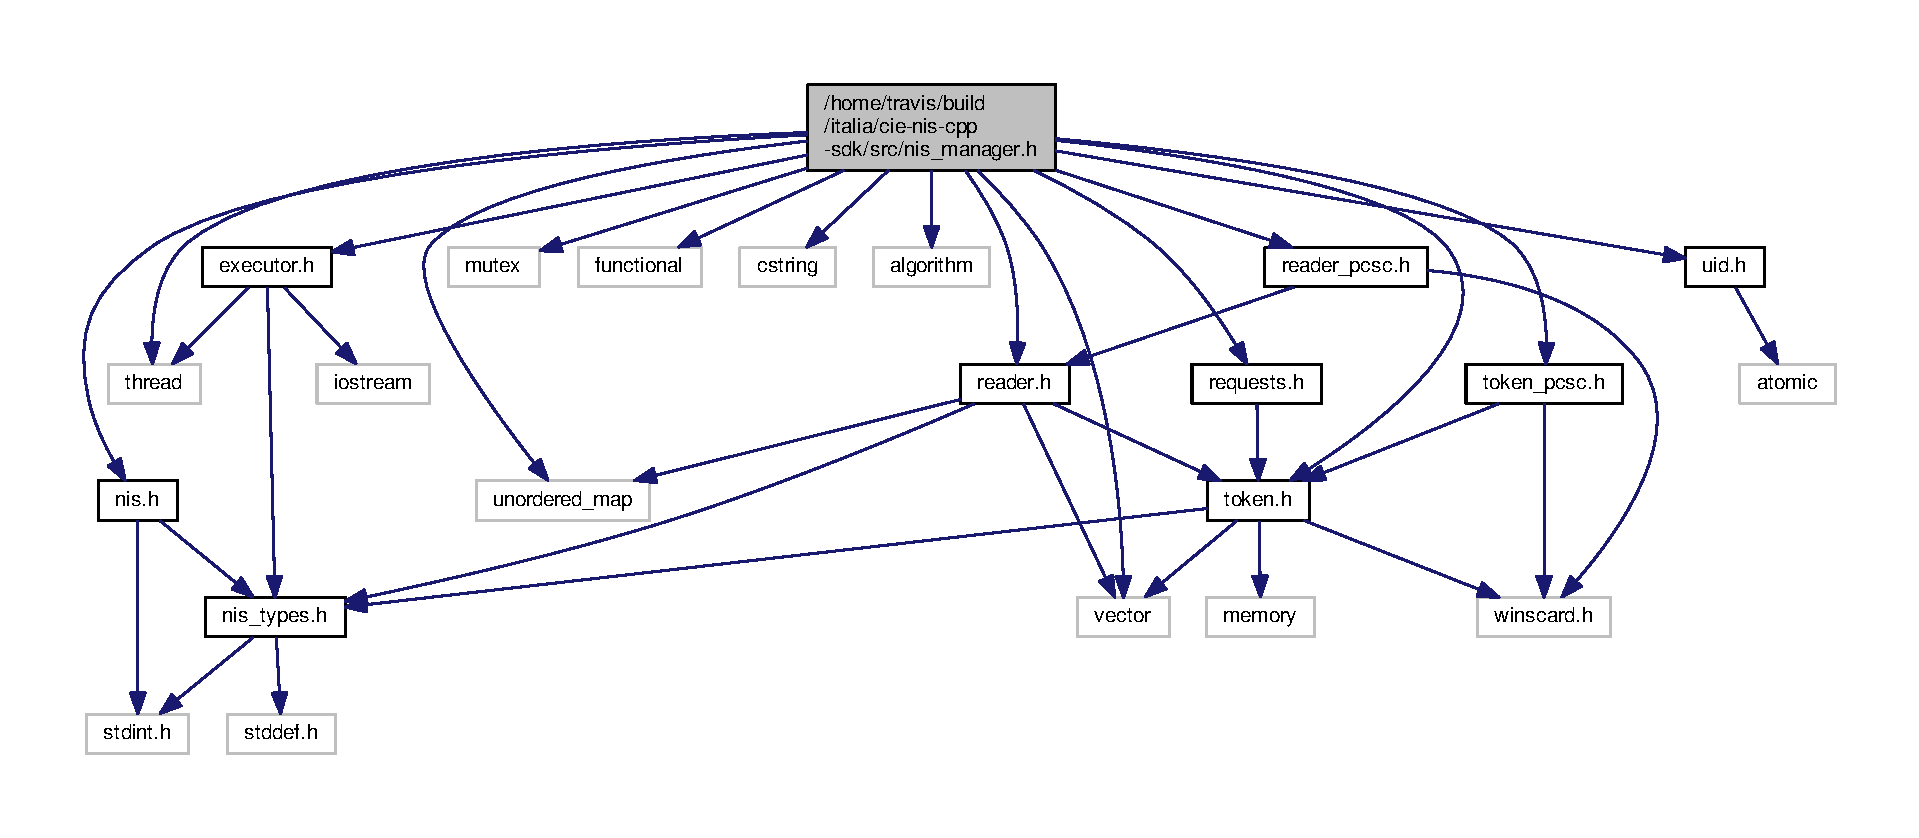
\includegraphics[width=350pt]{nis__manager_8h__incl}
\end{center}
\end{figure}
This graph shows which files directly or indirectly include this file\-:
\nopagebreak
\begin{figure}[H]
\begin{center}
\leavevmode
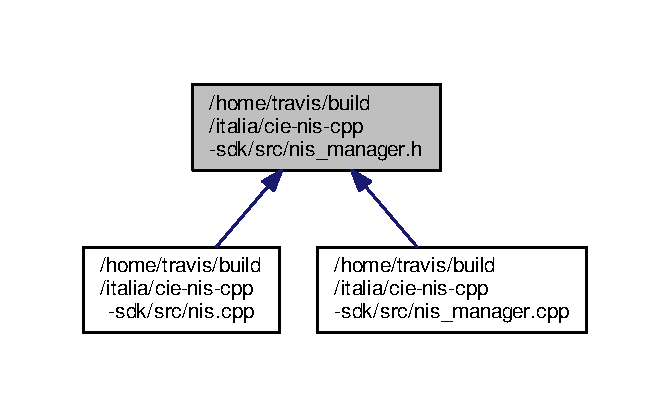
\includegraphics[width=321pt]{nis__manager_8h__dep__incl}
\end{center}
\end{figure}
\subsection*{Classes}
\begin{DoxyCompactItemize}
\item 
class \hyperlink{classNISManager}{N\-I\-S\-Manager}
\end{DoxyCompactItemize}


\subsection{Detailed Description}
N\-I\-S Manager. This file contains the declaration of teh N\-I\-S Manager, a singleton that provide facilities to manage backends, tokens and associated executors. 
\hypertarget{nis__types_8h}{\section{/home/travis/build/italia/cie-\/nis-\/cpp-\/sdk/src/nis\-\_\-types.h File Reference}
\label{nis__types_8h}\index{/home/travis/build/italia/cie-\/nis-\/cpp-\/sdk/src/nis\-\_\-types.\-h@{/home/travis/build/italia/cie-\/nis-\/cpp-\/sdk/src/nis\-\_\-types.\-h}}
}


N\-I\-S main header.  


{\ttfamily \#include $<$stddef.\-h$>$}\\*
{\ttfamily \#include $<$stdint.\-h$>$}\\*
Include dependency graph for nis\-\_\-types.\-h\-:
\nopagebreak
\begin{figure}[H]
\begin{center}
\leavevmode
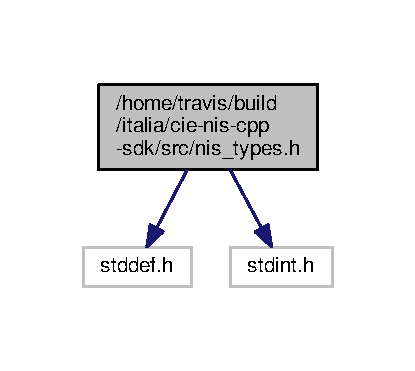
\includegraphics[width=199pt]{nis__types_8h__incl}
\end{center}
\end{figure}
This graph shows which files directly or indirectly include this file\-:
\nopagebreak
\begin{figure}[H]
\begin{center}
\leavevmode
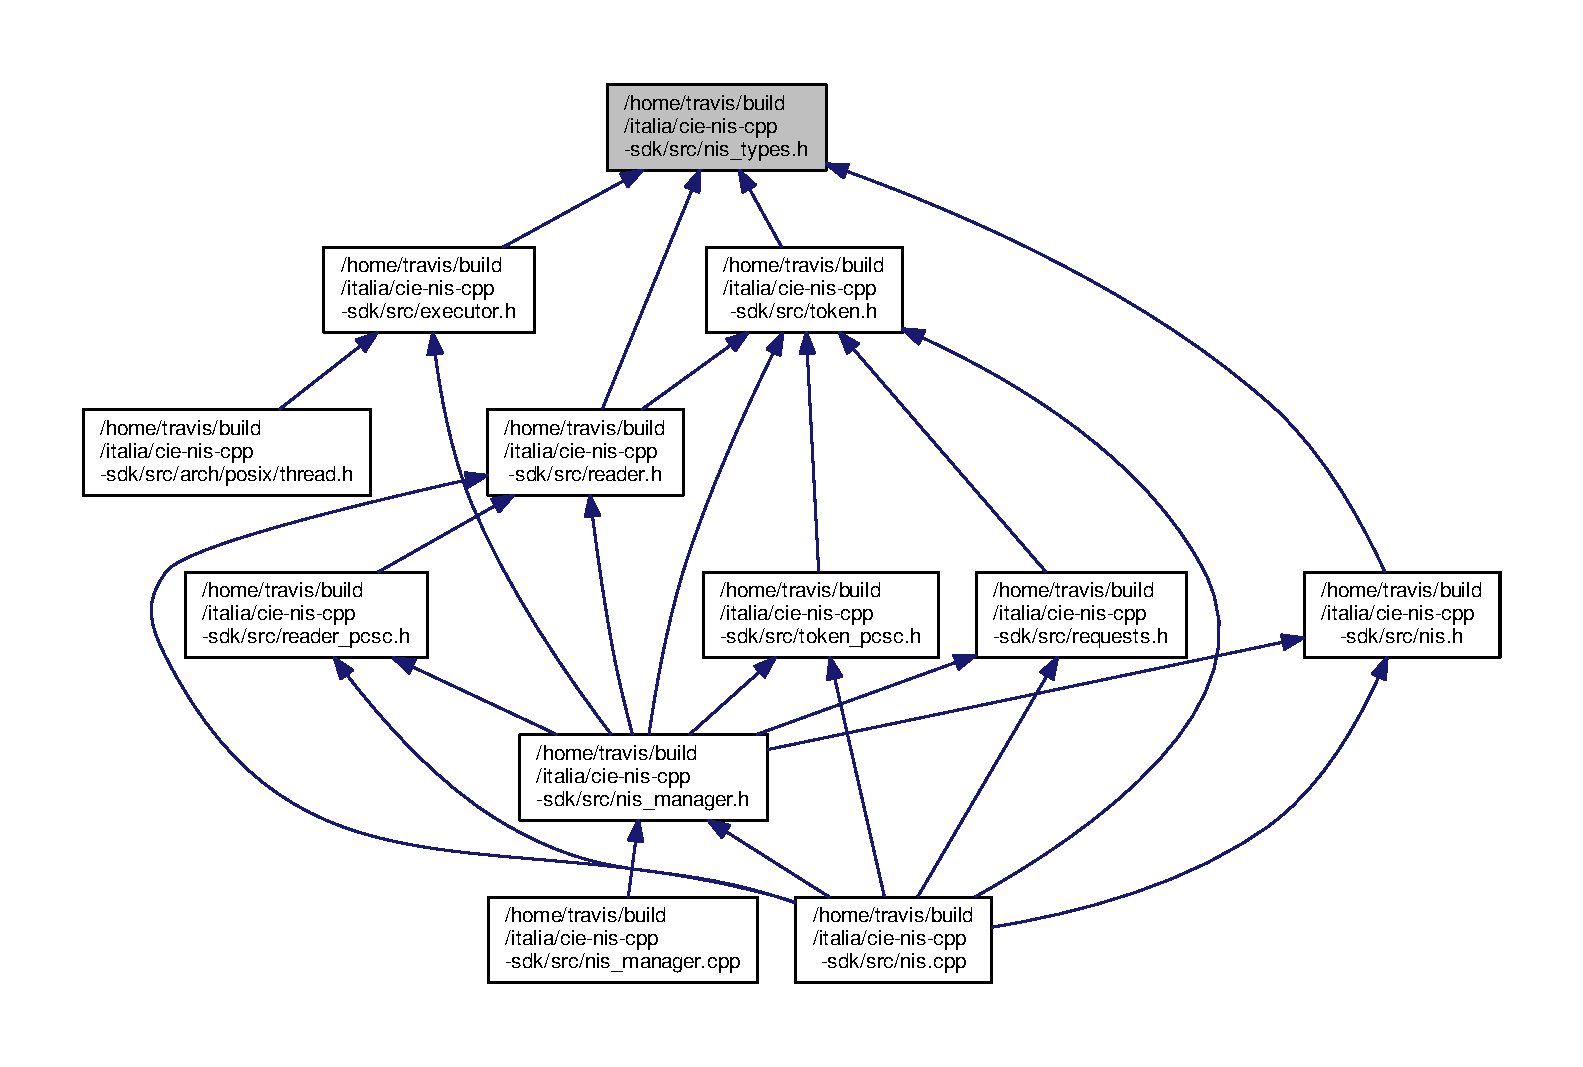
\includegraphics[width=350pt]{nis__types_8h__dep__incl}
\end{center}
\end{figure}
\subsection*{Macros}
\begin{DoxyCompactItemize}
\item 
\hypertarget{nis__types_8h_ab6a70fec3060f44922a3d93cd6b7623f}{\#define {\bfseries N\-I\-S\-\_\-\-L\-E\-N\-G\-T\-H}~12}\label{nis__types_8h_ab6a70fec3060f44922a3d93cd6b7623f}

\end{DoxyCompactItemize}
\subsection*{Typedefs}
\begin{DoxyCompactItemize}
\item 
typedef void $\ast$ \hyperlink{nis__types_8h_aeda8757494329f27e534f367b067eda3}{N\-I\-S\-Handle}
\item 
typedef void($\ast$ \hyperlink{nis__types_8h_a01a69b218db702baa14290be05ef112d}{nis\-\_\-callback\-\_\-t} )(char $\ast$const nis\-Data, size\-\_\-t len\-Data)
\end{DoxyCompactItemize}
\subsection*{Enumerations}
\begin{DoxyCompactItemize}
\item 
enum \hyperlink{nis__types_8h_a6ef53483e8ce2f8bc58bd1f75b3d0b38}{Tok\-Result} \{ \hyperlink{nis__types_8h_a6ef53483e8ce2f8bc58bd1f75b3d0b38af9c5076bc320f77c8fd8447b6892a3b5}{T\-O\-K\-\_\-\-R\-E\-S\-U\-L\-T\-\_\-\-O\-K}, 
\hyperlink{nis__types_8h_a6ef53483e8ce2f8bc58bd1f75b3d0b38aae636b718cda8835c66f85fad114362f}{T\-O\-K\-\_\-\-R\-E\-S\-U\-L\-T\-\_\-\-N\-O\-T\-\_\-\-C\-O\-N\-N\-E\-C\-T\-E\-D}, 
\hyperlink{nis__types_8h_a6ef53483e8ce2f8bc58bd1f75b3d0b38aca5238f4ea23a248dd5d87056e3e255a}{T\-O\-K\-\_\-\-R\-E\-S\-U\-L\-T\-\_\-\-R\-E\-A\-D\-\_\-\-E\-R\-R\-O\-R}, 
\hyperlink{nis__types_8h_a6ef53483e8ce2f8bc58bd1f75b3d0b38a8a7520e6e1ee16f45acc460ef0343e2a}{T\-O\-K\-\_\-\-R\-E\-S\-U\-L\-T\-\_\-\-G\-E\-N\-E\-R\-I\-C\-\_\-\-E\-R\-R\-O\-R}
 \}
\item 
enum \hyperlink{nis__types_8h_a484156f5b8cf43396c5bbe77226fa8da}{Reader\-Result} \{ \hyperlink{nis__types_8h_a484156f5b8cf43396c5bbe77226fa8daad9ba1cfa36627a40172f3b3099b3ef2b}{R\-E\-A\-D\-E\-R\-\_\-\-R\-E\-S\-U\-L\-T\-\_\-\-O\-K}, 
\hyperlink{nis__types_8h_a484156f5b8cf43396c5bbe77226fa8daafa0ff930e804f9dd92eef289af2eeb0a}{R\-E\-A\-D\-E\-R\-\_\-\-R\-E\-S\-U\-L\-T\-\_\-\-G\-E\-N\-E\-R\-I\-C\-\_\-\-E\-R\-R\-O\-R}
 \}
\item 
enum \hyperlink{nis__types_8h_acee299fbb7d897867808250049524594}{Backend\-Type} \{ \hyperlink{nis__types_8h_acee299fbb7d897867808250049524594a3ff60978c4e7dc38834c0e3758abbeab}{N\-I\-S\-\_\-\-B\-A\-C\-K\-E\-N\-D\-\_\-\-N\-O\-N\-E} = 0, 
\hyperlink{nis__types_8h_acee299fbb7d897867808250049524594a4090533bbae04dfb2aaae88b5ae40dff}{N\-I\-S\-\_\-\-B\-A\-C\-K\-E\-N\-D\-\_\-\-P\-C\-S\-C} = 1, 
\hyperlink{nis__types_8h_acee299fbb7d897867808250049524594ade11439a1cdb2e67e753e02b5fb3baaf}{N\-I\-S\-\_\-\-B\-A\-C\-K\-E\-N\-D\-\_\-\-A\-L\-L} = (N\-I\-S\-\_\-\-B\-A\-C\-K\-E\-N\-D\-\_\-\-P\-C\-S\-C)
 \}
\end{DoxyCompactItemize}


\subsection{Detailed Description}
N\-I\-S main header. Contains the return types and main types for N\-I\-S core functions. 

\subsection{Typedef Documentation}
\hypertarget{nis__types_8h_a01a69b218db702baa14290be05ef112d}{\index{nis\-\_\-types.\-h@{nis\-\_\-types.\-h}!nis\-\_\-callback\-\_\-t@{nis\-\_\-callback\-\_\-t}}
\index{nis\-\_\-callback\-\_\-t@{nis\-\_\-callback\-\_\-t}!nis_types.h@{nis\-\_\-types.\-h}}
\subsubsection[{nis\-\_\-callback\-\_\-t}]{\setlength{\rightskip}{0pt plus 5cm}typedef void($\ast$ nis\-\_\-callback\-\_\-t)(char $\ast$const nis\-Data, size\-\_\-t len\-Data)}}\label{nis__types_8h_a01a69b218db702baa14290be05ef112d}
Function pointer to a callback to be called when the N\-I\-S is being read from a token 
\begin{DoxyParams}{Parameters}
{\em nis\-Data} & pointer to the array that contains the N\-I\-S \\
\hline
{\em len\-Data} & size of {\itshape nis\-Data} \\
\hline
\end{DoxyParams}
\hypertarget{nis__types_8h_aeda8757494329f27e534f367b067eda3}{\index{nis\-\_\-types.\-h@{nis\-\_\-types.\-h}!N\-I\-S\-Handle@{N\-I\-S\-Handle}}
\index{N\-I\-S\-Handle@{N\-I\-S\-Handle}!nis_types.h@{nis\-\_\-types.\-h}}
\subsubsection[{N\-I\-S\-Handle}]{\setlength{\rightskip}{0pt plus 5cm}typedef void$\ast$ {\bf N\-I\-S\-Handle}}}\label{nis__types_8h_aeda8757494329f27e534f367b067eda3}
An handler to refer to a specific instance of a token 

\subsection{Enumeration Type Documentation}
\hypertarget{nis__types_8h_acee299fbb7d897867808250049524594}{\index{nis\-\_\-types.\-h@{nis\-\_\-types.\-h}!Backend\-Type@{Backend\-Type}}
\index{Backend\-Type@{Backend\-Type}!nis_types.h@{nis\-\_\-types.\-h}}
\subsubsection[{Backend\-Type}]{\setlength{\rightskip}{0pt plus 5cm}enum {\bf Backend\-Type}}}\label{nis__types_8h_acee299fbb7d897867808250049524594}
\begin{Desc}
\item[Enumerator]\par
\begin{description}
\index{N\-I\-S\-\_\-\-B\-A\-C\-K\-E\-N\-D\-\_\-\-N\-O\-N\-E@{N\-I\-S\-\_\-\-B\-A\-C\-K\-E\-N\-D\-\_\-\-N\-O\-N\-E}!nis\-\_\-types.\-h@{nis\-\_\-types.\-h}}\index{nis\-\_\-types.\-h@{nis\-\_\-types.\-h}!N\-I\-S\-\_\-\-B\-A\-C\-K\-E\-N\-D\-\_\-\-N\-O\-N\-E@{N\-I\-S\-\_\-\-B\-A\-C\-K\-E\-N\-D\-\_\-\-N\-O\-N\-E}}\item[{\em 
\hypertarget{nis__types_8h_acee299fbb7d897867808250049524594a3ff60978c4e7dc38834c0e3758abbeab}{N\-I\-S\-\_\-\-B\-A\-C\-K\-E\-N\-D\-\_\-\-N\-O\-N\-E}\label{nis__types_8h_acee299fbb7d897867808250049524594a3ff60978c4e7dc38834c0e3758abbeab}
}]No backend selected \index{N\-I\-S\-\_\-\-B\-A\-C\-K\-E\-N\-D\-\_\-\-P\-C\-S\-C@{N\-I\-S\-\_\-\-B\-A\-C\-K\-E\-N\-D\-\_\-\-P\-C\-S\-C}!nis\-\_\-types.\-h@{nis\-\_\-types.\-h}}\index{nis\-\_\-types.\-h@{nis\-\_\-types.\-h}!N\-I\-S\-\_\-\-B\-A\-C\-K\-E\-N\-D\-\_\-\-P\-C\-S\-C@{N\-I\-S\-\_\-\-B\-A\-C\-K\-E\-N\-D\-\_\-\-P\-C\-S\-C}}\item[{\em 
\hypertarget{nis__types_8h_acee299fbb7d897867808250049524594a4090533bbae04dfb2aaae88b5ae40dff}{N\-I\-S\-\_\-\-B\-A\-C\-K\-E\-N\-D\-\_\-\-P\-C\-S\-C}\label{nis__types_8h_acee299fbb7d897867808250049524594a4090533bbae04dfb2aaae88b5ae40dff}
}]P\-C\-S\-C backend \index{N\-I\-S\-\_\-\-B\-A\-C\-K\-E\-N\-D\-\_\-\-A\-L\-L@{N\-I\-S\-\_\-\-B\-A\-C\-K\-E\-N\-D\-\_\-\-A\-L\-L}!nis\-\_\-types.\-h@{nis\-\_\-types.\-h}}\index{nis\-\_\-types.\-h@{nis\-\_\-types.\-h}!N\-I\-S\-\_\-\-B\-A\-C\-K\-E\-N\-D\-\_\-\-A\-L\-L@{N\-I\-S\-\_\-\-B\-A\-C\-K\-E\-N\-D\-\_\-\-A\-L\-L}}\item[{\em 
\hypertarget{nis__types_8h_acee299fbb7d897867808250049524594ade11439a1cdb2e67e753e02b5fb3baaf}{N\-I\-S\-\_\-\-B\-A\-C\-K\-E\-N\-D\-\_\-\-A\-L\-L}\label{nis__types_8h_acee299fbb7d897867808250049524594ade11439a1cdb2e67e753e02b5fb3baaf}
}]All available backends \end{description}
\end{Desc}
\hypertarget{nis__types_8h_a484156f5b8cf43396c5bbe77226fa8da}{\index{nis\-\_\-types.\-h@{nis\-\_\-types.\-h}!Reader\-Result@{Reader\-Result}}
\index{Reader\-Result@{Reader\-Result}!nis_types.h@{nis\-\_\-types.\-h}}
\subsubsection[{Reader\-Result}]{\setlength{\rightskip}{0pt plus 5cm}enum {\bf Reader\-Result}}}\label{nis__types_8h_a484156f5b8cf43396c5bbe77226fa8da}
\begin{Desc}
\item[Enumerator]\par
\begin{description}
\index{R\-E\-A\-D\-E\-R\-\_\-\-R\-E\-S\-U\-L\-T\-\_\-\-O\-K@{R\-E\-A\-D\-E\-R\-\_\-\-R\-E\-S\-U\-L\-T\-\_\-\-O\-K}!nis\-\_\-types.\-h@{nis\-\_\-types.\-h}}\index{nis\-\_\-types.\-h@{nis\-\_\-types.\-h}!R\-E\-A\-D\-E\-R\-\_\-\-R\-E\-S\-U\-L\-T\-\_\-\-O\-K@{R\-E\-A\-D\-E\-R\-\_\-\-R\-E\-S\-U\-L\-T\-\_\-\-O\-K}}\item[{\em 
\hypertarget{nis__types_8h_a484156f5b8cf43396c5bbe77226fa8daad9ba1cfa36627a40172f3b3099b3ef2b}{R\-E\-A\-D\-E\-R\-\_\-\-R\-E\-S\-U\-L\-T\-\_\-\-O\-K}\label{nis__types_8h_a484156f5b8cf43396c5bbe77226fa8daad9ba1cfa36627a40172f3b3099b3ef2b}
}]Success \index{R\-E\-A\-D\-E\-R\-\_\-\-R\-E\-S\-U\-L\-T\-\_\-\-G\-E\-N\-E\-R\-I\-C\-\_\-\-E\-R\-R\-O\-R@{R\-E\-A\-D\-E\-R\-\_\-\-R\-E\-S\-U\-L\-T\-\_\-\-G\-E\-N\-E\-R\-I\-C\-\_\-\-E\-R\-R\-O\-R}!nis\-\_\-types.\-h@{nis\-\_\-types.\-h}}\index{nis\-\_\-types.\-h@{nis\-\_\-types.\-h}!R\-E\-A\-D\-E\-R\-\_\-\-R\-E\-S\-U\-L\-T\-\_\-\-G\-E\-N\-E\-R\-I\-C\-\_\-\-E\-R\-R\-O\-R@{R\-E\-A\-D\-E\-R\-\_\-\-R\-E\-S\-U\-L\-T\-\_\-\-G\-E\-N\-E\-R\-I\-C\-\_\-\-E\-R\-R\-O\-R}}\item[{\em 
\hypertarget{nis__types_8h_a484156f5b8cf43396c5bbe77226fa8daafa0ff930e804f9dd92eef289af2eeb0a}{R\-E\-A\-D\-E\-R\-\_\-\-R\-E\-S\-U\-L\-T\-\_\-\-G\-E\-N\-E\-R\-I\-C\-\_\-\-E\-R\-R\-O\-R}\label{nis__types_8h_a484156f5b8cf43396c5bbe77226fa8daafa0ff930e804f9dd92eef289af2eeb0a}
}]Some error has occurred \end{description}
\end{Desc}
\hypertarget{nis__types_8h_a6ef53483e8ce2f8bc58bd1f75b3d0b38}{\index{nis\-\_\-types.\-h@{nis\-\_\-types.\-h}!Tok\-Result@{Tok\-Result}}
\index{Tok\-Result@{Tok\-Result}!nis_types.h@{nis\-\_\-types.\-h}}
\subsubsection[{Tok\-Result}]{\setlength{\rightskip}{0pt plus 5cm}enum {\bf Tok\-Result}}}\label{nis__types_8h_a6ef53483e8ce2f8bc58bd1f75b3d0b38}
\begin{Desc}
\item[Enumerator]\par
\begin{description}
\index{T\-O\-K\-\_\-\-R\-E\-S\-U\-L\-T\-\_\-\-O\-K@{T\-O\-K\-\_\-\-R\-E\-S\-U\-L\-T\-\_\-\-O\-K}!nis\-\_\-types.\-h@{nis\-\_\-types.\-h}}\index{nis\-\_\-types.\-h@{nis\-\_\-types.\-h}!T\-O\-K\-\_\-\-R\-E\-S\-U\-L\-T\-\_\-\-O\-K@{T\-O\-K\-\_\-\-R\-E\-S\-U\-L\-T\-\_\-\-O\-K}}\item[{\em 
\hypertarget{nis__types_8h_a6ef53483e8ce2f8bc58bd1f75b3d0b38af9c5076bc320f77c8fd8447b6892a3b5}{T\-O\-K\-\_\-\-R\-E\-S\-U\-L\-T\-\_\-\-O\-K}\label{nis__types_8h_a6ef53483e8ce2f8bc58bd1f75b3d0b38af9c5076bc320f77c8fd8447b6892a3b5}
}]Success \index{T\-O\-K\-\_\-\-R\-E\-S\-U\-L\-T\-\_\-\-N\-O\-T\-\_\-\-C\-O\-N\-N\-E\-C\-T\-E\-D@{T\-O\-K\-\_\-\-R\-E\-S\-U\-L\-T\-\_\-\-N\-O\-T\-\_\-\-C\-O\-N\-N\-E\-C\-T\-E\-D}!nis\-\_\-types.\-h@{nis\-\_\-types.\-h}}\index{nis\-\_\-types.\-h@{nis\-\_\-types.\-h}!T\-O\-K\-\_\-\-R\-E\-S\-U\-L\-T\-\_\-\-N\-O\-T\-\_\-\-C\-O\-N\-N\-E\-C\-T\-E\-D@{T\-O\-K\-\_\-\-R\-E\-S\-U\-L\-T\-\_\-\-N\-O\-T\-\_\-\-C\-O\-N\-N\-E\-C\-T\-E\-D}}\item[{\em 
\hypertarget{nis__types_8h_a6ef53483e8ce2f8bc58bd1f75b3d0b38aae636b718cda8835c66f85fad114362f}{T\-O\-K\-\_\-\-R\-E\-S\-U\-L\-T\-\_\-\-N\-O\-T\-\_\-\-C\-O\-N\-N\-E\-C\-T\-E\-D}\label{nis__types_8h_a6ef53483e8ce2f8bc58bd1f75b3d0b38aae636b718cda8835c66f85fad114362f}
}]No card connected \index{T\-O\-K\-\_\-\-R\-E\-S\-U\-L\-T\-\_\-\-R\-E\-A\-D\-\_\-\-E\-R\-R\-O\-R@{T\-O\-K\-\_\-\-R\-E\-S\-U\-L\-T\-\_\-\-R\-E\-A\-D\-\_\-\-E\-R\-R\-O\-R}!nis\-\_\-types.\-h@{nis\-\_\-types.\-h}}\index{nis\-\_\-types.\-h@{nis\-\_\-types.\-h}!T\-O\-K\-\_\-\-R\-E\-S\-U\-L\-T\-\_\-\-R\-E\-A\-D\-\_\-\-E\-R\-R\-O\-R@{T\-O\-K\-\_\-\-R\-E\-S\-U\-L\-T\-\_\-\-R\-E\-A\-D\-\_\-\-E\-R\-R\-O\-R}}\item[{\em 
\hypertarget{nis__types_8h_a6ef53483e8ce2f8bc58bd1f75b3d0b38aca5238f4ea23a248dd5d87056e3e255a}{T\-O\-K\-\_\-\-R\-E\-S\-U\-L\-T\-\_\-\-R\-E\-A\-D\-\_\-\-E\-R\-R\-O\-R}\label{nis__types_8h_a6ef53483e8ce2f8bc58bd1f75b3d0b38aca5238f4ea23a248dd5d87056e3e255a}
}]Cannot read from the card \index{T\-O\-K\-\_\-\-R\-E\-S\-U\-L\-T\-\_\-\-G\-E\-N\-E\-R\-I\-C\-\_\-\-E\-R\-R\-O\-R@{T\-O\-K\-\_\-\-R\-E\-S\-U\-L\-T\-\_\-\-G\-E\-N\-E\-R\-I\-C\-\_\-\-E\-R\-R\-O\-R}!nis\-\_\-types.\-h@{nis\-\_\-types.\-h}}\index{nis\-\_\-types.\-h@{nis\-\_\-types.\-h}!T\-O\-K\-\_\-\-R\-E\-S\-U\-L\-T\-\_\-\-G\-E\-N\-E\-R\-I\-C\-\_\-\-E\-R\-R\-O\-R@{T\-O\-K\-\_\-\-R\-E\-S\-U\-L\-T\-\_\-\-G\-E\-N\-E\-R\-I\-C\-\_\-\-E\-R\-R\-O\-R}}\item[{\em 
\hypertarget{nis__types_8h_a6ef53483e8ce2f8bc58bd1f75b3d0b38a8a7520e6e1ee16f45acc460ef0343e2a}{T\-O\-K\-\_\-\-R\-E\-S\-U\-L\-T\-\_\-\-G\-E\-N\-E\-R\-I\-C\-\_\-\-E\-R\-R\-O\-R}\label{nis__types_8h_a6ef53483e8ce2f8bc58bd1f75b3d0b38a8a7520e6e1ee16f45acc460ef0343e2a}
}]Some error has occurred \end{description}
\end{Desc}

\hypertarget{reader_8h}{\section{/home/travis/build/italia/cie-\/nis-\/cpp-\/sdk/src/reader.h File Reference}
\label{reader_8h}\index{/home/travis/build/italia/cie-\/nis-\/cpp-\/sdk/src/reader.\-h@{/home/travis/build/italia/cie-\/nis-\/cpp-\/sdk/src/reader.\-h}}
}


A Reader.  


{\ttfamily \#include $<$vector$>$}\\*
{\ttfamily \#include $<$unordered\-\_\-map$>$}\\*
{\ttfamily \#include \char`\"{}nis\-\_\-types.\-h\char`\"{}}\\*
{\ttfamily \#include \char`\"{}token.\-h\char`\"{}}\\*
Include dependency graph for reader.\-h\-:
\nopagebreak
\begin{figure}[H]
\begin{center}
\leavevmode
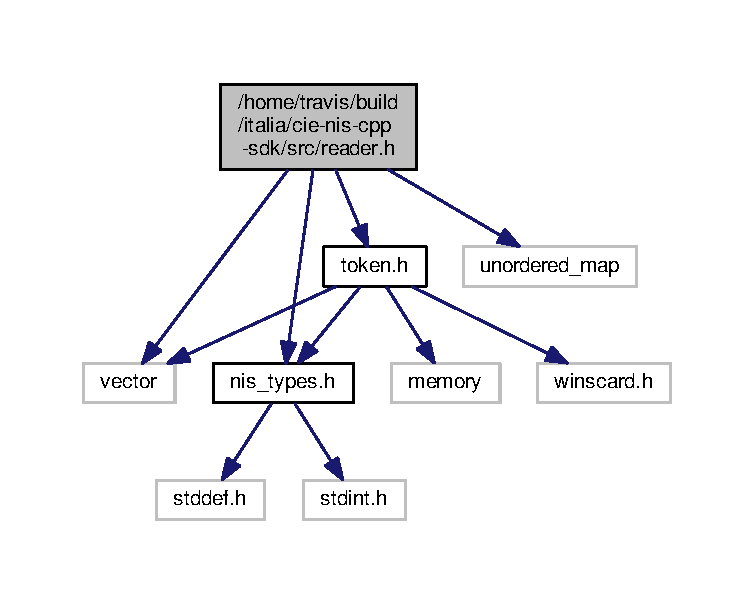
\includegraphics[width=350pt]{reader_8h__incl}
\end{center}
\end{figure}
This graph shows which files directly or indirectly include this file\-:
\nopagebreak
\begin{figure}[H]
\begin{center}
\leavevmode
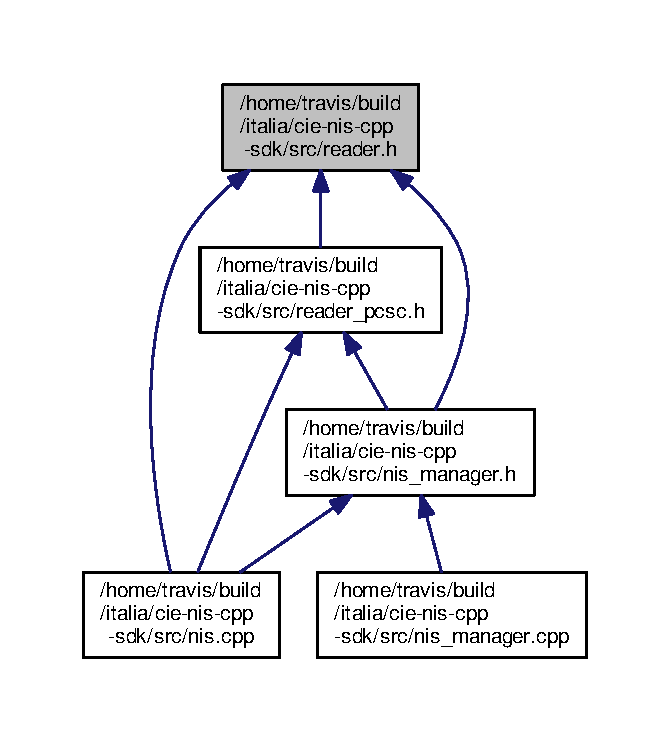
\includegraphics[width=321pt]{reader_8h__dep__incl}
\end{center}
\end{figure}
\subsection*{Classes}
\begin{DoxyCompactItemize}
\item 
class \hyperlink{classcie_1_1nis_1_1Reader}{cie\-::nis\-::\-Reader}
\end{DoxyCompactItemize}


\subsection{Detailed Description}
A Reader. This file contains the declaration of a base Reader. In this library, the words 'Reader' and 'Backend' are used almost interchangeably, meaning that a Reador or a Backend is a system that can exchange information with a Token (i.\-e. a card) via a specific protocol (e.\-g. P\-C\-S\-C compatible reader). A Reader is responsible for high-\/level facilities like enumerating the connected readers that are compatible with the backend it implements and to provide a reference to a named \-::\-Token. This calss is abstract and need to be extended in order to provide a specific implementation. Usually for each Reader's subclass there is a corresponding Token's subclass. \begin{DoxySeeAlso}{See Also}
Reader\-P\-C\-S\-C 

Token\-P\-C\-S\-C 
\end{DoxySeeAlso}

\hypertarget{token_8h}{\section{/home/travis/build/italia/cie-\/nis-\/cpp-\/sdk/src/token.h File Reference}
\label{token_8h}\index{/home/travis/build/italia/cie-\/nis-\/cpp-\/sdk/src/token.\-h@{/home/travis/build/italia/cie-\/nis-\/cpp-\/sdk/src/token.\-h}}
}


A Token.  


{\ttfamily \#include $<$vector$>$}\\*
{\ttfamily \#include $<$memory$>$}\\*
{\ttfamily \#include $<$winscard.\-h$>$}\\*
{\ttfamily \#include \char`\"{}nis\-\_\-types.\-h\char`\"{}}\\*
Include dependency graph for token.\-h\-:
\nopagebreak
\begin{figure}[H]
\begin{center}
\leavevmode
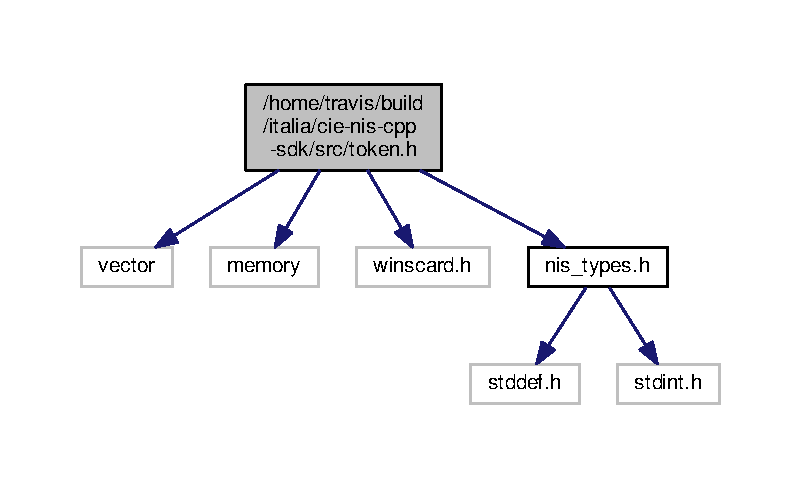
\includegraphics[width=350pt]{token_8h__incl}
\end{center}
\end{figure}
This graph shows which files directly or indirectly include this file\-:
\nopagebreak
\begin{figure}[H]
\begin{center}
\leavevmode
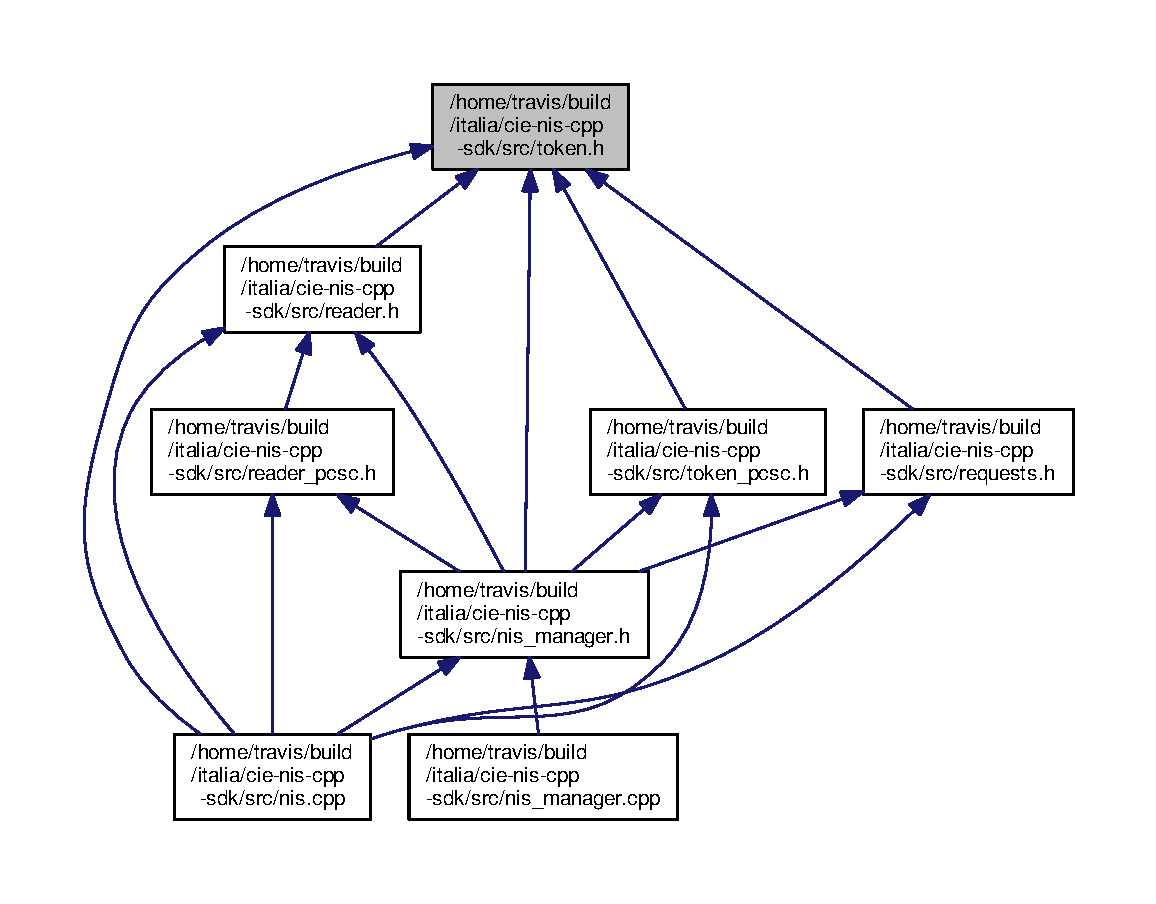
\includegraphics[width=350pt]{token_8h__dep__incl}
\end{center}
\end{figure}
\subsection*{Classes}
\begin{DoxyCompactItemize}
\item 
class \hyperlink{classnis_1_1interface_1_1Token}{nis\-::interface\-::\-Token}
\end{DoxyCompactItemize}


\subsection{Detailed Description}
A Token. A Token represents a card or token with which a Reader can interact. It's main use is to connect/disconnect and to transmit/receive data packets to/from a card. This is an abstract class meaning that it must be extended to provide the funcionality of a specific protocol (e.\-g. P\-C\-S\-C). Usually for each Token's subclass there is a corresponding Reader's subclass. \begin{DoxySeeAlso}{See Also}
Token\-P\-C\-S\-C 

Reader\-P\-C\-S\-C 
\end{DoxySeeAlso}

%--- End generated contents ---

% Index
\newpage
\phantomsection
\addcontentsline{toc}{chapter}{Index}
\printindex

\end{document}
